% Compile from the paper directory with:
%   latexmk -lualatex research_summary_for_slides.tex
% or:
%   lualatex research_summary_for_slides.tex
\documentclass[aspectratio=169,10pt]{beamer}

\usepackage{luatexja}
\usepackage[haranoaji]{luatexja-preset}
\usepackage{amsmath,amssymb,booktabs,array}
\usepackage{graphicx}
\usepackage{xcolor}

\usetheme{Madrid}
\usecolortheme{dolphin}
\setbeamertemplate{navigation symbols}{}
\setbeamertemplate{caption}[numbered]
\setbeamerfont{caption}{size=\scriptsize}
\setbeamerfont{footnote}{size=\tiny}
\setbeamersize{text margin left=7mm,text margin right=7mm}

\definecolor{accent}{RGB}{29,78,121}
\definecolor{good}{RGB}{31,122,70}
\definecolor{warn}{RGB}{176,92,25}
\setbeamercolor{structure}{fg=accent}
\setbeamercolor{alerted text}{fg=warn}

\graphicspath{{slide_assets/}{evidence_figures/}{evidence_figures/application_dags/}{results_report/figures/}{../results/method_comparison_figures/RESULT_stg/}{../results/method_comparison_figures/result_BENCHMARK/}}

\newcommand{\code}[1]{\texttt{#1}}
\newcommand{\best}[1]{\textcolor{good}{\bfseries #1}}
\newcommand{\caution}[1]{\textcolor{warn}{\bfseries #1}}

\title[CUDA Stream配置とSM資源配分]{単一GPU上のStatic Task Graph実行における\\CUDA Stream配置とSM資源配分}
\subtitle{DAG構造と実カーネル特性に基づく二段階ヒューリスティック}
\author{}
\institute{}
\date{}

\begin{document}

\begin{frame}
  \titlepage
\end{frame}

\begin{frame}{背景：Streamを増やすだけでは速くならない}
  \begin{columns}[T,onlytextwidth]
    \begin{column}{0.53\textwidth}
      \begin{itemize}
        \item 独立なCUDAカーネルは複数Streamで同時実行できる
        \item 一方、複数Streamは同じGPUのSMを共有する
        \item 重要な先行タスクの遅延は、後続処理全体へ伝播する
        \item 起動・同期・Green Context管理にもコストがある
      \end{itemize}
    \end{column}
    \begin{column}{0.43\textwidth}
      \begin{block}{理想化した実行時間の下界}
        \[
          T \geq \max\!\left(\frac{W}{M},\,CP\right)
        \]
        \small
        $W$: 総仕事量，$M$: SM数，$CP$: クリティカルパス長
      \end{block}
      \begin{alertblock}{課題}
        並列性だけでなく、依存関係とSM競合を同時に考える必要がある。
      \end{alertblock}
    \end{column}
  \end{columns}
\end{frame}

\begin{frame}{研究目的と検証項目}
  \begin{block}{目的}
    Static Task Graph（STG）のDAG構造と実カーネル特性から、
    Stream配置とSM資源配分を決める方式が\alert{どの条件で有効か}を明らかにする。
  \end{block}
  \begin{enumerate}
    \item 複数Streamによるタスク並列性は実行時間短縮に寄与するか
    \item bottom levelによる重要度付けとSM配分は既存方式を改善するか
    \item DAG構造の違いは、提案方式の効果をどう変えるか
  \end{enumerate}
  \vspace{2mm}
  \begin{exampleblock}{事前仮説}
    独立分岐が多いDAGでは複数Streamが効きやすい。
    長い分岐が合流するDAGでは、遅い分岐と合流待ちが性能を支配する。
  \end{exampleblock}
\end{frame}

\begin{frame}{提案手法：二段階ヒューリスティック}
  \begin{columns}[T,onlytextwidth]
    \begin{column}{0.23\textwidth}
      \begin{block}{入力}
        \centering
        STG\\[1mm]
        依存関係 $E$\\
        代表時間 $p_i$\\
        SM別実測 $g_i(x)$
      \end{block}
    \end{column}
    \begin{column}{0.05\textwidth}
      \centering\vspace{13mm}$\Longrightarrow$
    \end{column}
    \begin{column}{0.28\textwidth}
      \begin{block}{Stage 1：Stream配置}
        \begin{enumerate}
          \item bottom level計算
          \item readyタスクを優先
          \item 最早終了Streamへ配置
        \end{enumerate}
      \end{block}
    \end{column}
    \begin{column}{0.05\textwidth}
      \centering\vspace{13mm}$\Longrightarrow$
    \end{column}
    \begin{column}{0.30\textwidth}
      \begin{block}{Stage 2：SM配分}
        \begin{enumerate}
          \item Stream配置を固定
          \item 8 SM単位で候補生成
          \item 予測makespan最小を選択
        \end{enumerate}
      \end{block}
    \end{column}
  \end{columns}
  \vspace{2mm}
  \small 最後に、決定した構成で\alert{実CUDAカーネル}を起動し、CUDA Eventで評価する。
\end{frame}

\begin{frame}{STGは実カーネルと一対一に対応}
  \begin{columns}[T,onlytextwidth]
    \begin{column}{0.48\textwidth}
      \begin{itemize}
        \item タスクIDをランチャ・依存関係・SMプロファイル・出力検証で共有
        \item \code{proc\_time}は固定条件で測った実カーネルの代表時間
        \item SM数 $8,16,\ldots,64$ ごとに実測曲線 $g_i(x)$ を作成
        \item DAGは実行トレースからの自動抽出ではなく、実装のデータ依存から静的に定義
      \end{itemize}
      \begin{block}{3種類の時間を区別}
        \scriptsize
        \begin{tabular}{@{}ll@{}}
          \toprule
          値 & 用途 \\
          \midrule
          $p_i$ & bottom level・初期配置 \\
          $g_i(x)$ & SM配分候補の予測 \\
          \code{gpu\_kernel\_ms} & 最終性能評価 \\
          \bottomrule
        \end{tabular}
      \end{block}
    \end{column}
    \begin{column}{0.49\textwidth}
      \centering
      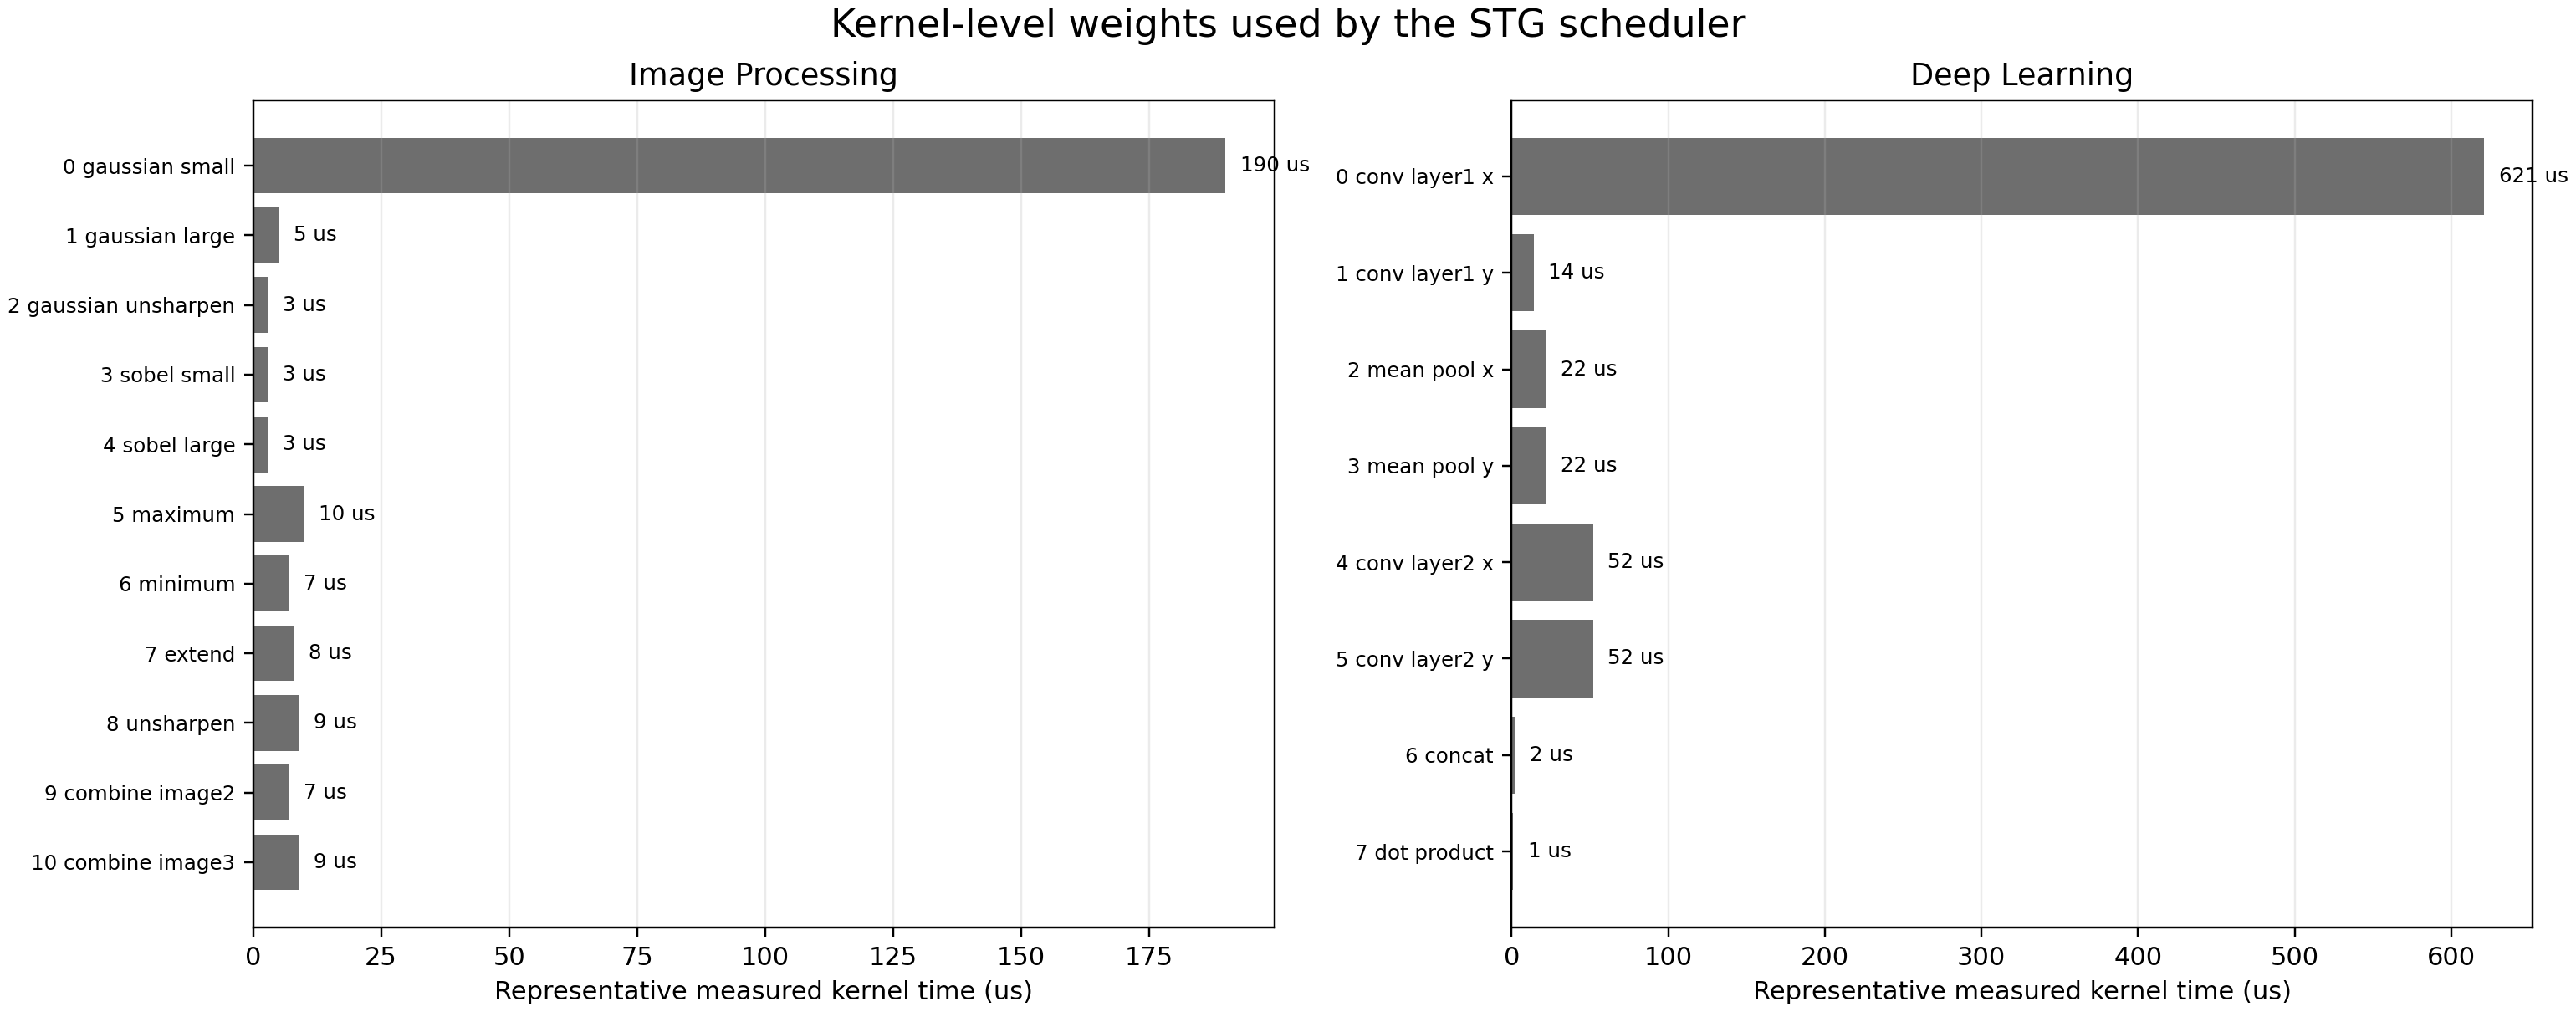
\includegraphics[width=\linewidth,height=0.72\textheight,keepaspectratio]{kernel_measurement_mapping.png}
    \end{column}
  \end{columns}
\end{frame}

\begin{frame}{重要度・Stream配置・SM配分の定式化}
  \small
  \begin{columns}[T,onlytextwidth]
    \begin{column}{0.32\textwidth}
      \begin{block}{bottom level}
        \[
        b_i = p_i +
        \begin{cases}
          0 & (S_i=\emptyset)\\
          \max_{j\in S_i} b_j & (\text{otherwise})
        \end{cases}
        \]
        $b_i$が大きいreadyタスクを優先する。
      \end{block}
    \end{column}
    \begin{column}{0.32\textwidth}
      \begin{block}{Stream配置}
        \[
          r_i=\max_{j\in P_i} f_j
        \]
        \[
          f(i,s)=e(i,s)+p_i
        \]
        予測終了時刻が最小となるStreamへ配置する。
      \end{block}
    \end{column}
    \begin{column}{0.32\textwidth}
      \begin{block}{SM配分}
        \[
          L_s=\sum_{\sigma(i)=s}\hat p_i(x_s)
        \]
        \[
          \hat C=\max_s L_s
        \]
        $\hat p_i(x_s)=g_i(x_s)$を用い、$\hat C$最小の候補を選ぶ。
      \end{block}
    \end{column}
  \end{columns}
  \begin{alertblock}{モデルの限界}
    予測値は、依存待ち・同時実行時の性能変化・起動同期・Context解放を完全には表さない。
  \end{alertblock}
\end{frame}

\begin{frame}{関連研究における位置付け}
  \small
  \begin{columns}[T,onlytextwidth]
    \begin{column}{0.55\textwidth}
      \begin{block}{直接比較すべき手法}
        \begin{enumerate}
          \item \textbf{HEFT}：upward rankと挿入型EFT
          \item \textbf{PEFT}：後続コストを含む実行先選択
          \item \textbf{CPOP}：クリティカルパス重視
          \item \textbf{DLS / HLFET / ETF}：DAGリストスケジューリング
          \item \textbf{SSGS}：eligible集合から最早資源可行位置へ配置
        \end{enumerate}
      \end{block}
    \end{column}
    \begin{column}{0.42\textwidth}
      \begin{alertblock}{本手法との主要な差}
        既存のDAG方式は主に\alert{タスク--プロセッサ割当て}を決める。
        本手法はHEFT型の配置を単一GPU内へ適用した後、配置を固定して
        \alert{Stream数とStream別SM数}を探索する。
      \end{alertblock}
      \begin{exampleblock}{比較対象ではなく類推に留まる分野}
        EDF、WFQ、DRF、DSATUR、勤務表GAなどは、優先度または資源共有の
        一部だけが類似し、同一問題のベースラインではない。
      \end{exampleblock}
    \end{column}
  \end{columns}
\end{frame}

\begin{frame}{実験条件}
  \begin{columns}[T,onlytextwidth]
    \begin{column}{0.48\textwidth}
      \begin{block}{比較する4手法}
        \begin{enumerate}
          \item Sequential
          \item Existing
          \item Existing + Green Context
          \item Proposed
        \end{enumerate}
      \end{block}
      \begin{block}{合成STG（5種類）}
        Fully Parallel、Mixed、Multiple Long Branches、Random DAG、Sequential Chain
      \end{block}
    \end{column}
    \begin{column}{0.48\textwidth}
      \begin{block}{実アプリケーション（6種類）}
        Vector Square、Black--Scholes、Machine Learning、HITS、Image Processing、Deep Learning
      \end{block}
      \begin{block}{測定}
        \begin{itemize}
          \item 33回実行、先頭3回をウォームアップとして除外
          \item 30サンプルの平均・標準偏差・中央値・95\%信頼区間
          \item 主指標：CUDA Eventによる\code{gpu\_kernel\_ms}
          \item 実アプリケーションは出力値も検証
        \end{itemize}
      \end{block}
    \end{column}
  \end{columns}
\end{frame}

\begin{frame}{結果1：合成STGでは全5種類でProposedが最短}
  \centering
  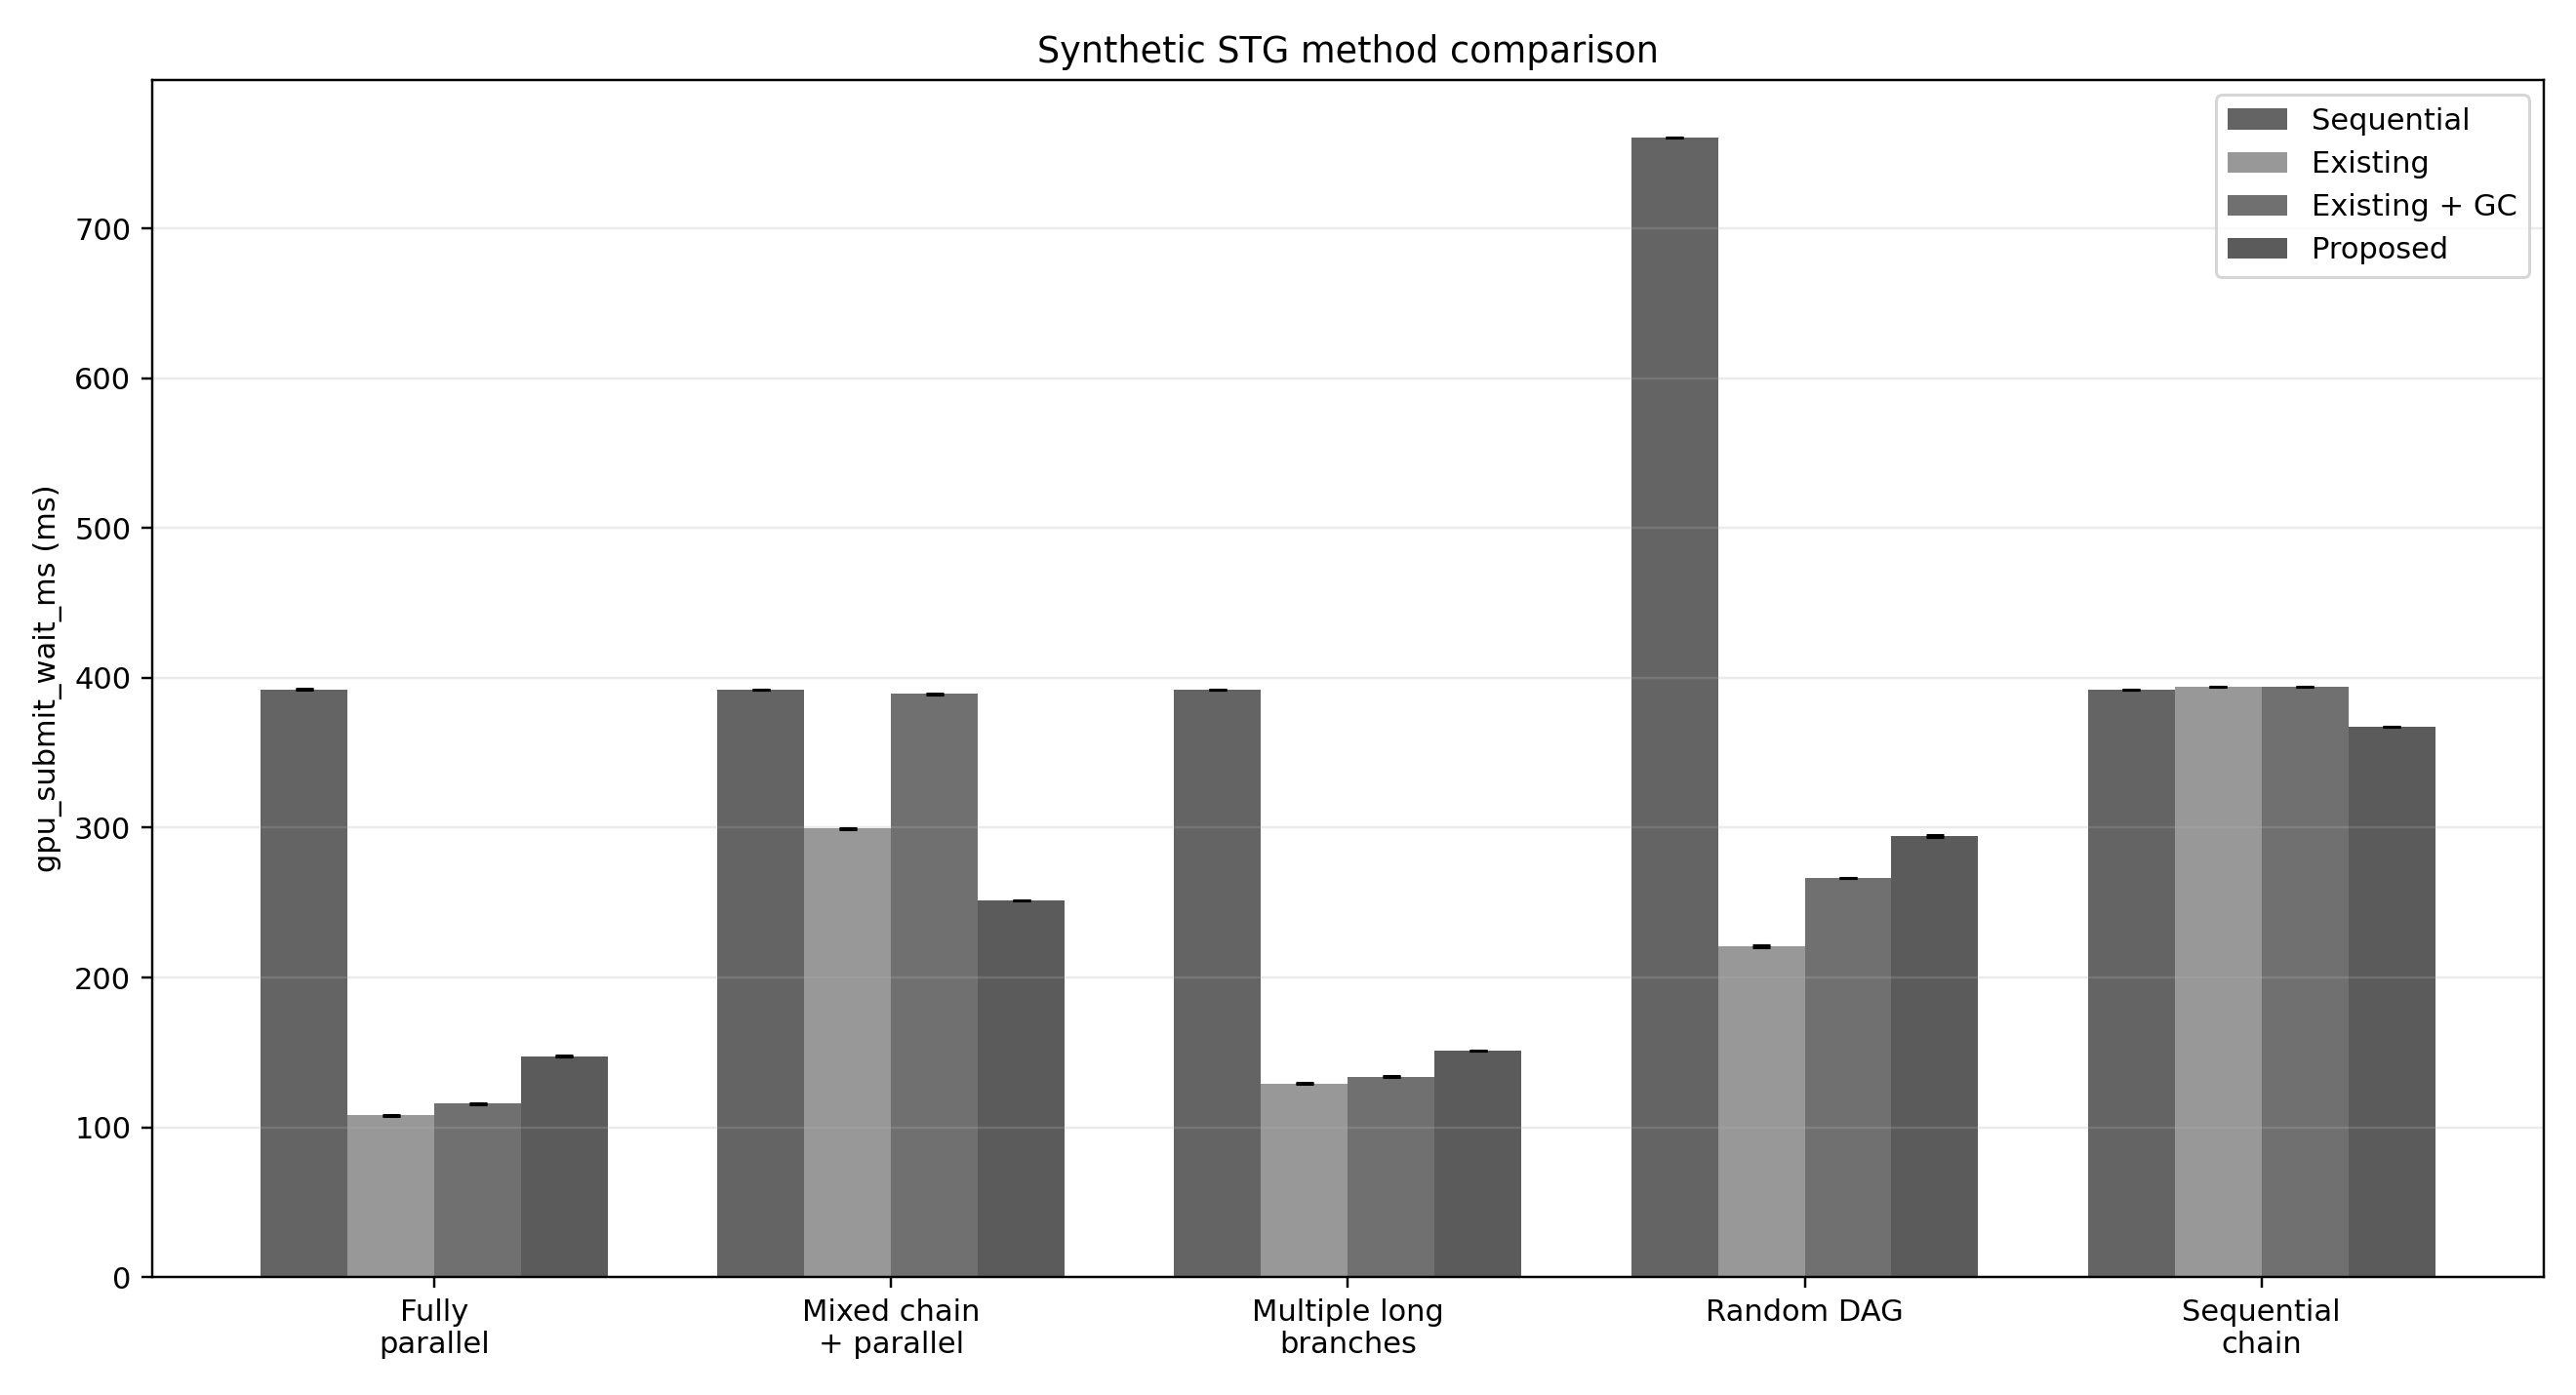
\includegraphics[width=0.94\linewidth,height=0.72\textheight,keepaspectratio]{synthetic_method_comparison.png}
  \vspace{-1mm}
  \begin{alertblock}{解釈}
    \small 合成STGでの優位性を、実アプリケーションや異なるGPUへそのまま一般化はできない。
  \end{alertblock}
\end{frame}

\begin{frame}{結果2：実アプリケーションでは最良手法が異なる}
  \centering
  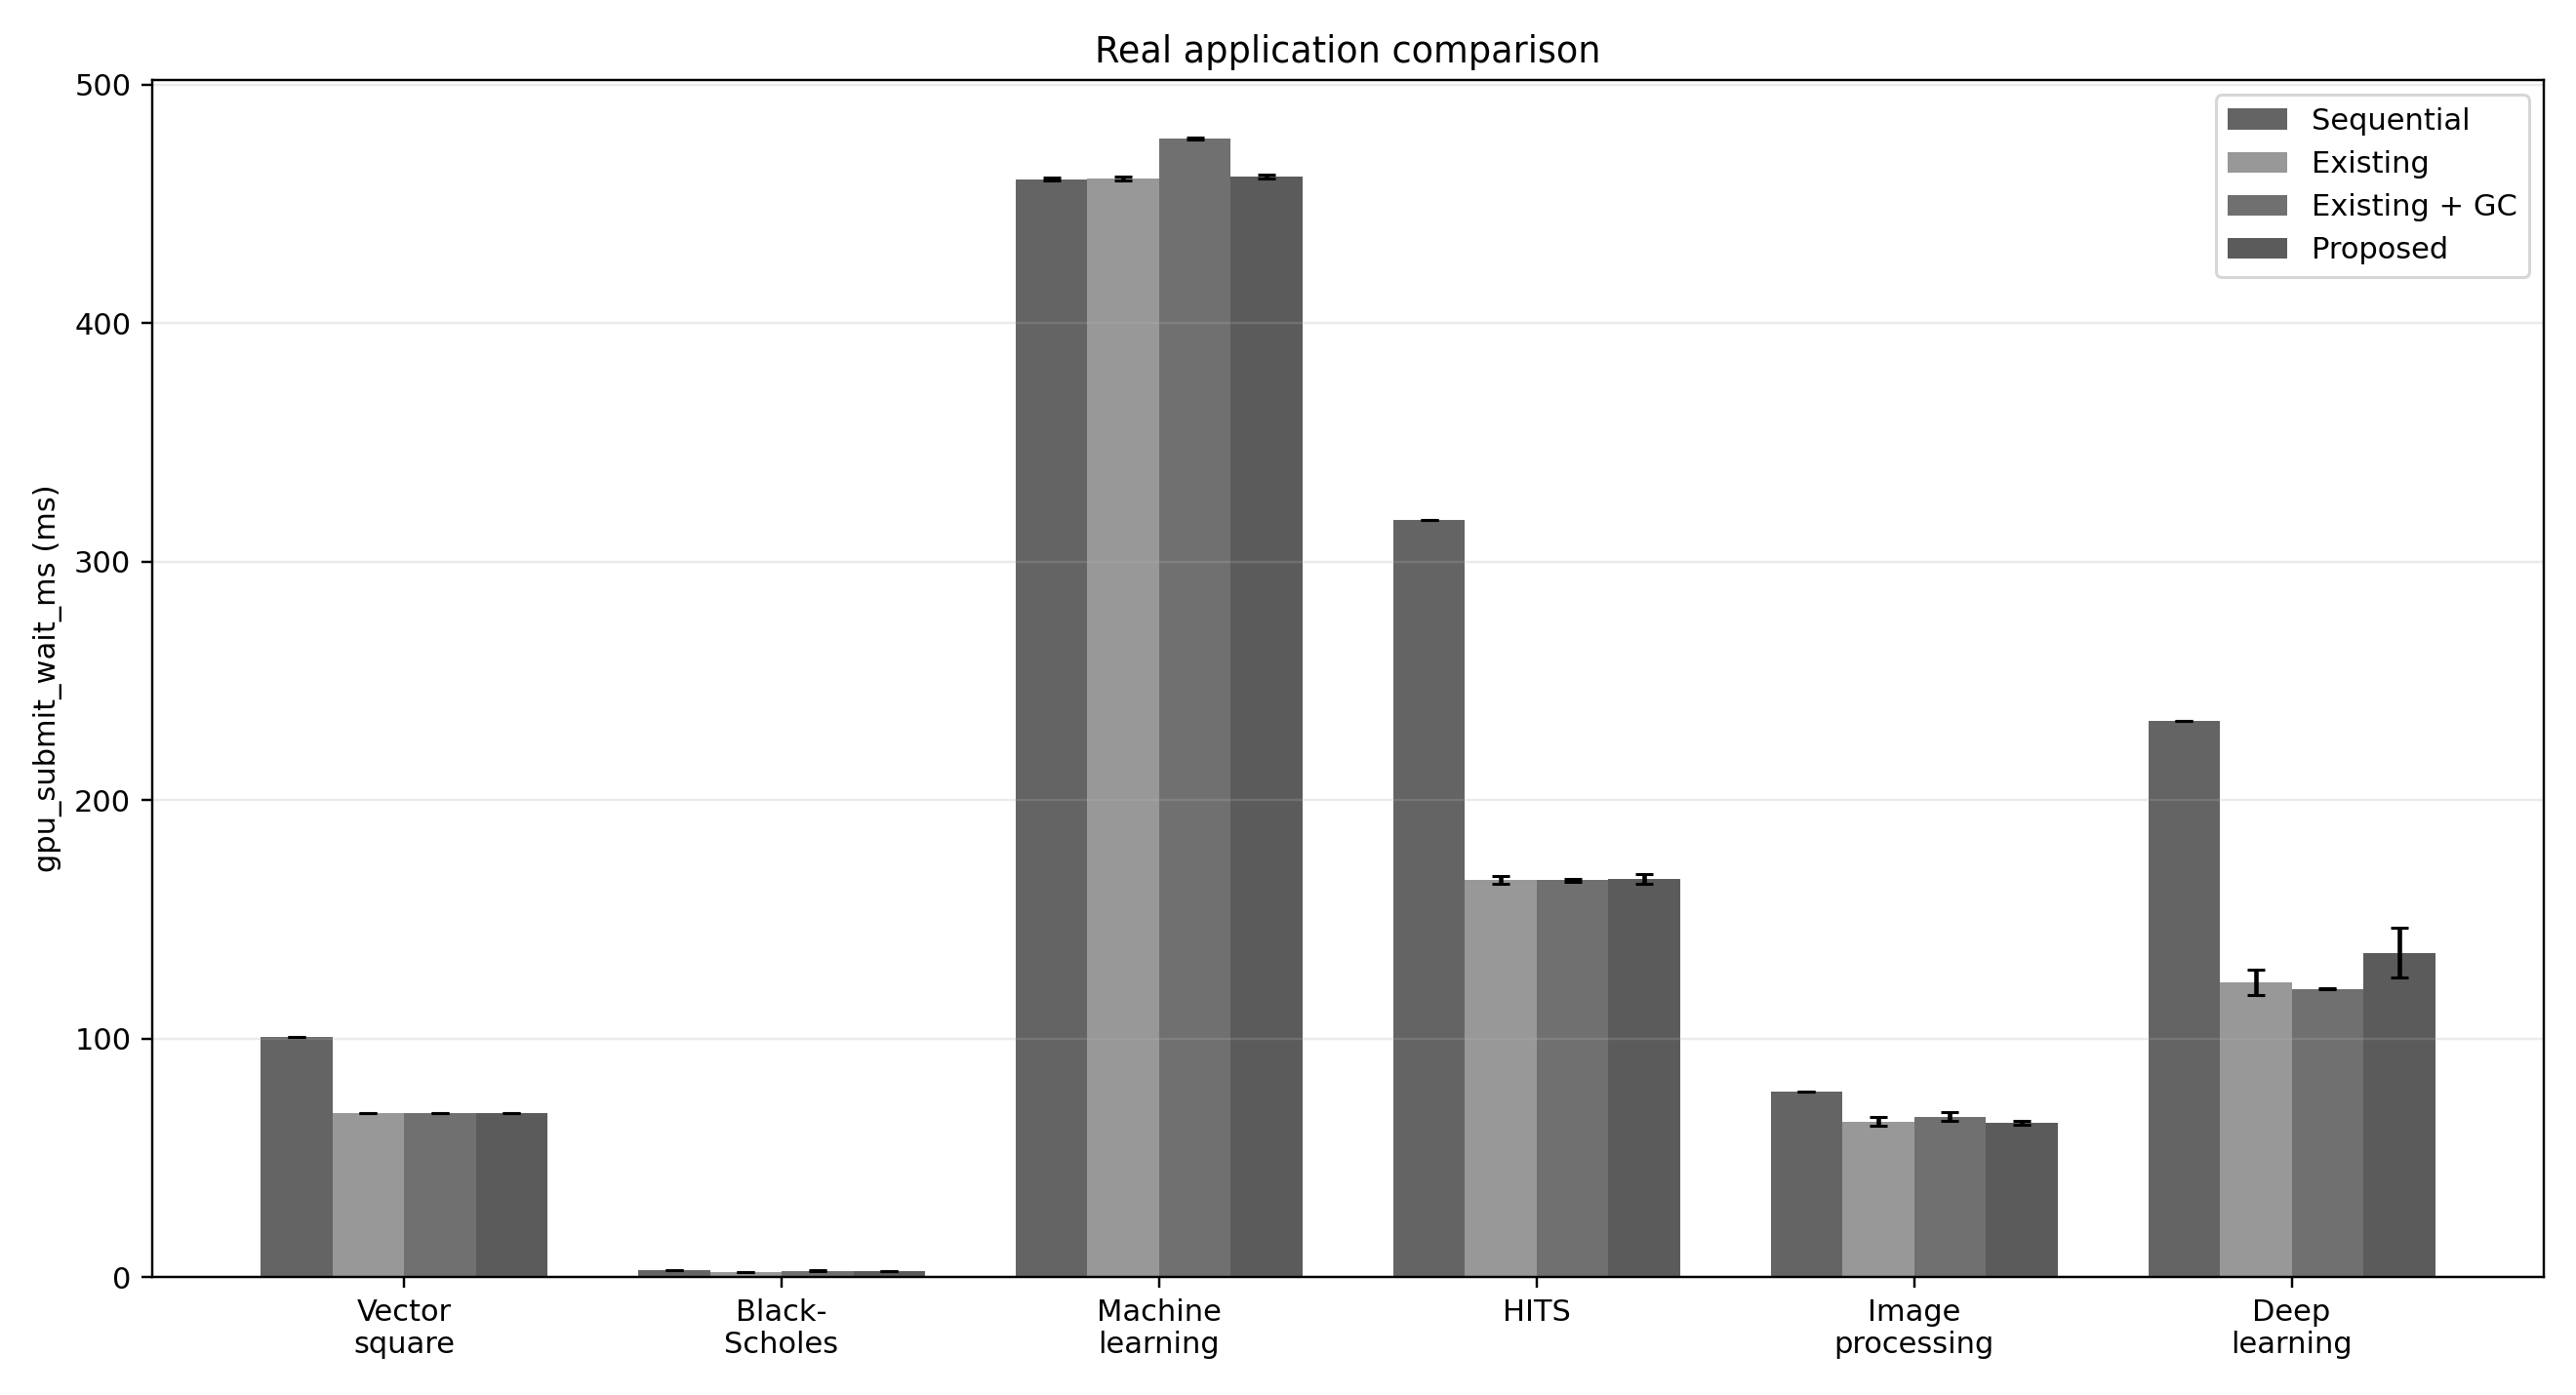
\includegraphics[width=0.91\linewidth,height=0.65\textheight,keepaspectratio]{real_application_four_methods.png}
  \vspace{-1mm}
  \begin{columns}[T,onlytextwidth]
    \begin{column}{0.48\textwidth}
      \small
      \textbf{Proposedが最短：} Image Processing（64.32 ms）
    \end{column}
    \begin{column}{0.48\textwidth}
      \small
      \textbf{Existingが最短：} Vector Square、Black--Scholes、Deep Learning
    \end{column}
  \end{columns}
  \vspace{1mm}
  \caution{HITSのExistingとProposedは数値検証FAILのため、性能主張から除外。}
\end{frame}

\begin{frame}{Image ProcessingとDeep Learning：DAG構造の違い}
  \begin{columns}[T,onlytextwidth]
    \begin{column}{0.49\textwidth}
      \centering
      \textbf{Image Processing}\\[-1mm]
      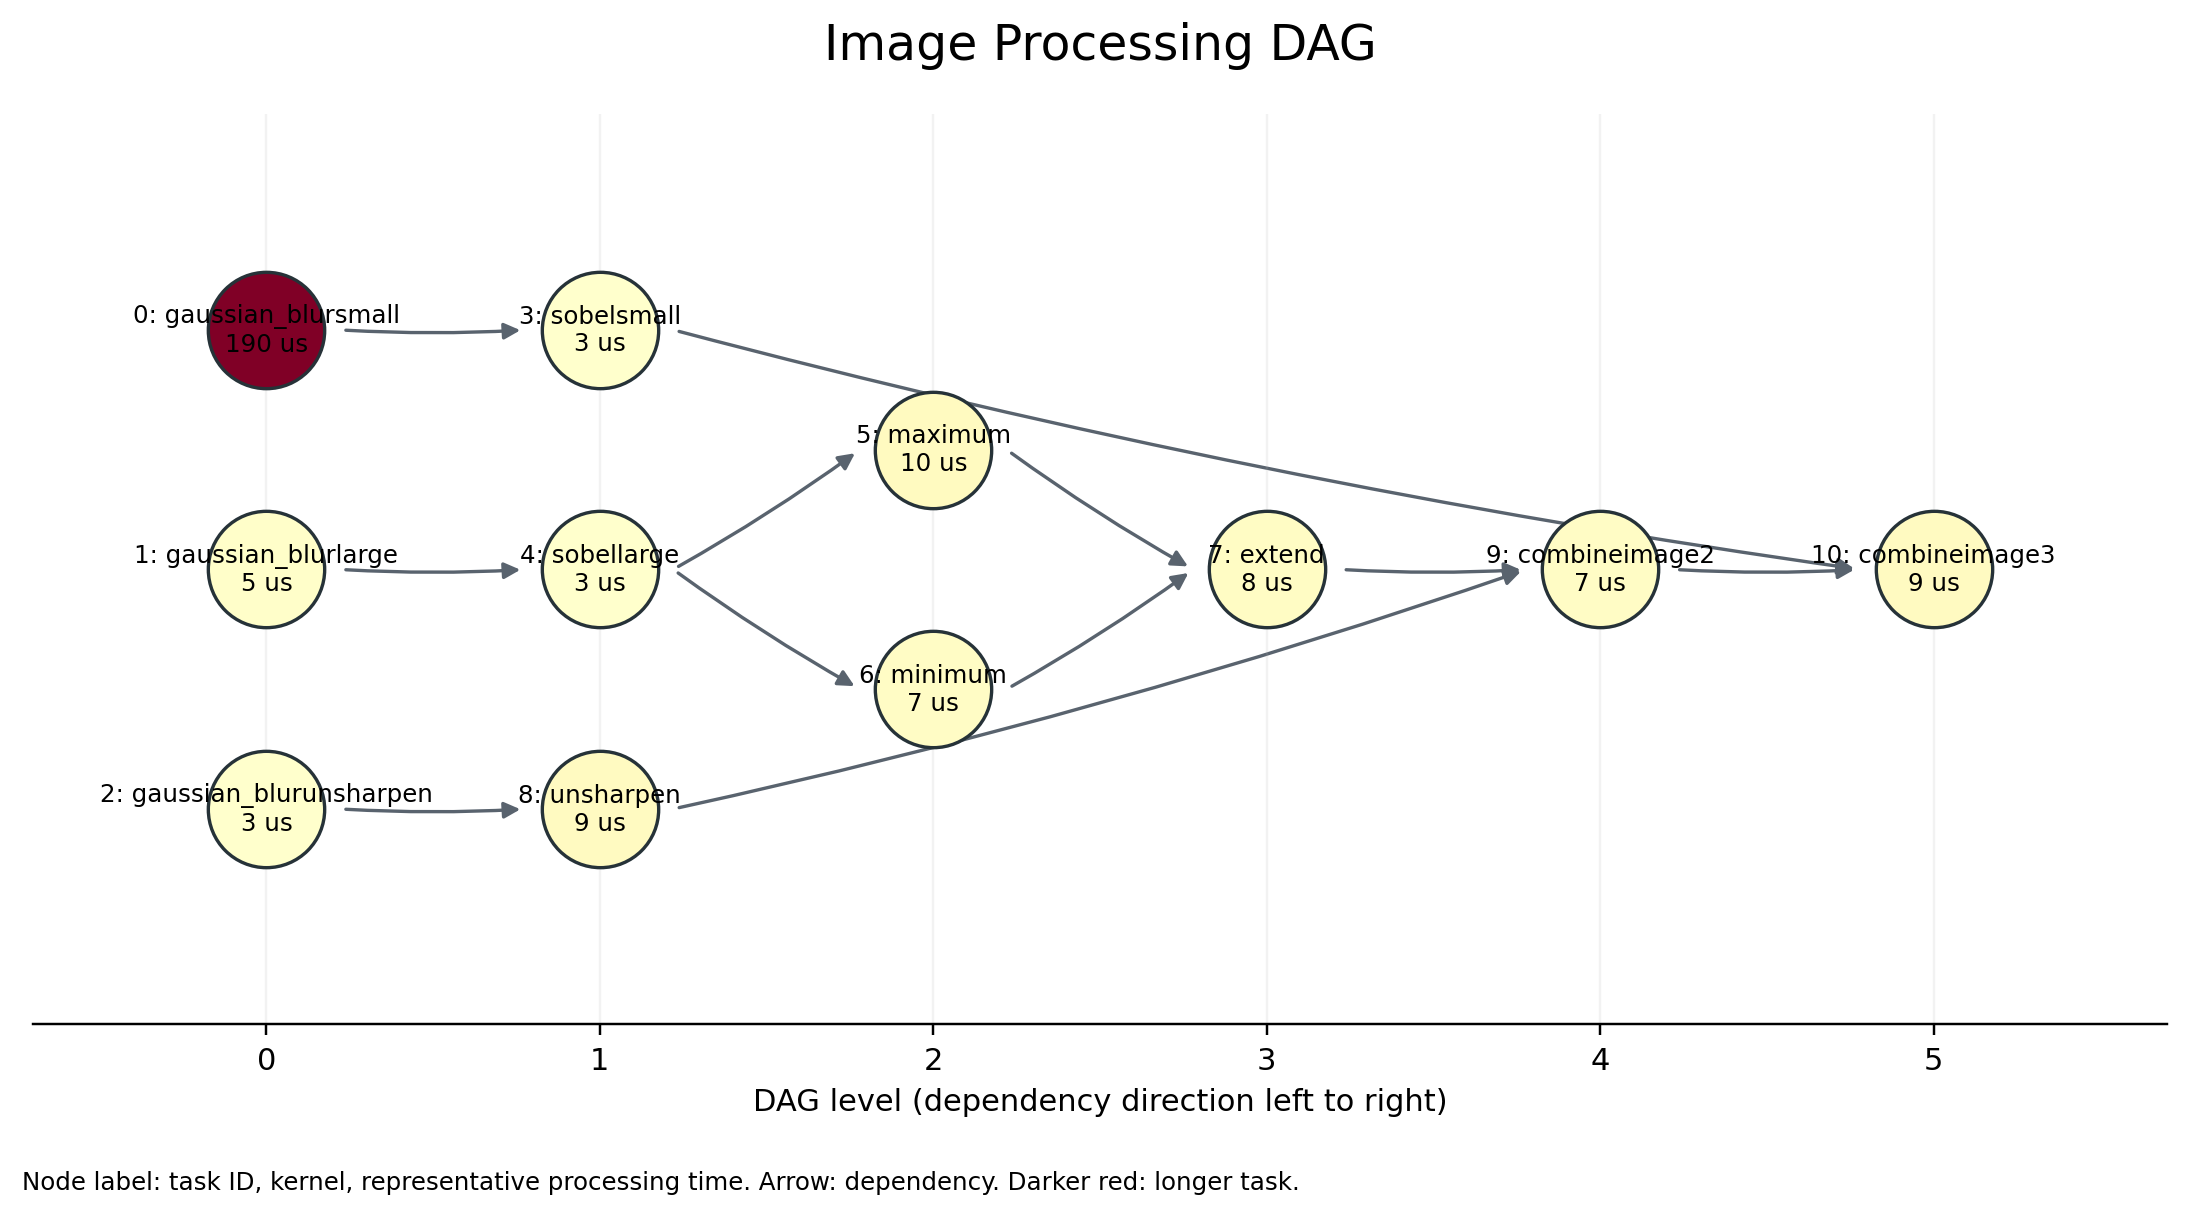
\includegraphics[width=\linewidth,height=0.43\textheight,keepaspectratio]{image_processing_dag.png}
      \scriptsize
      \begin{tabular}{@{}lr@{}}
        根タスク数 / 最大幅 & 3 / 3 \\
        $W$ / $CP$ & 254 / 202 \\
        並列度上限 $W/CP$ & 1.26 \\
      \end{tabular}
      \par\smallskip
      \small 複数の独立分岐をStreamへ分散しやすい。
    \end{column}
    \begin{column}{0.49\textwidth}
      \centering
      \textbf{Deep Learning}\\[-1mm]
      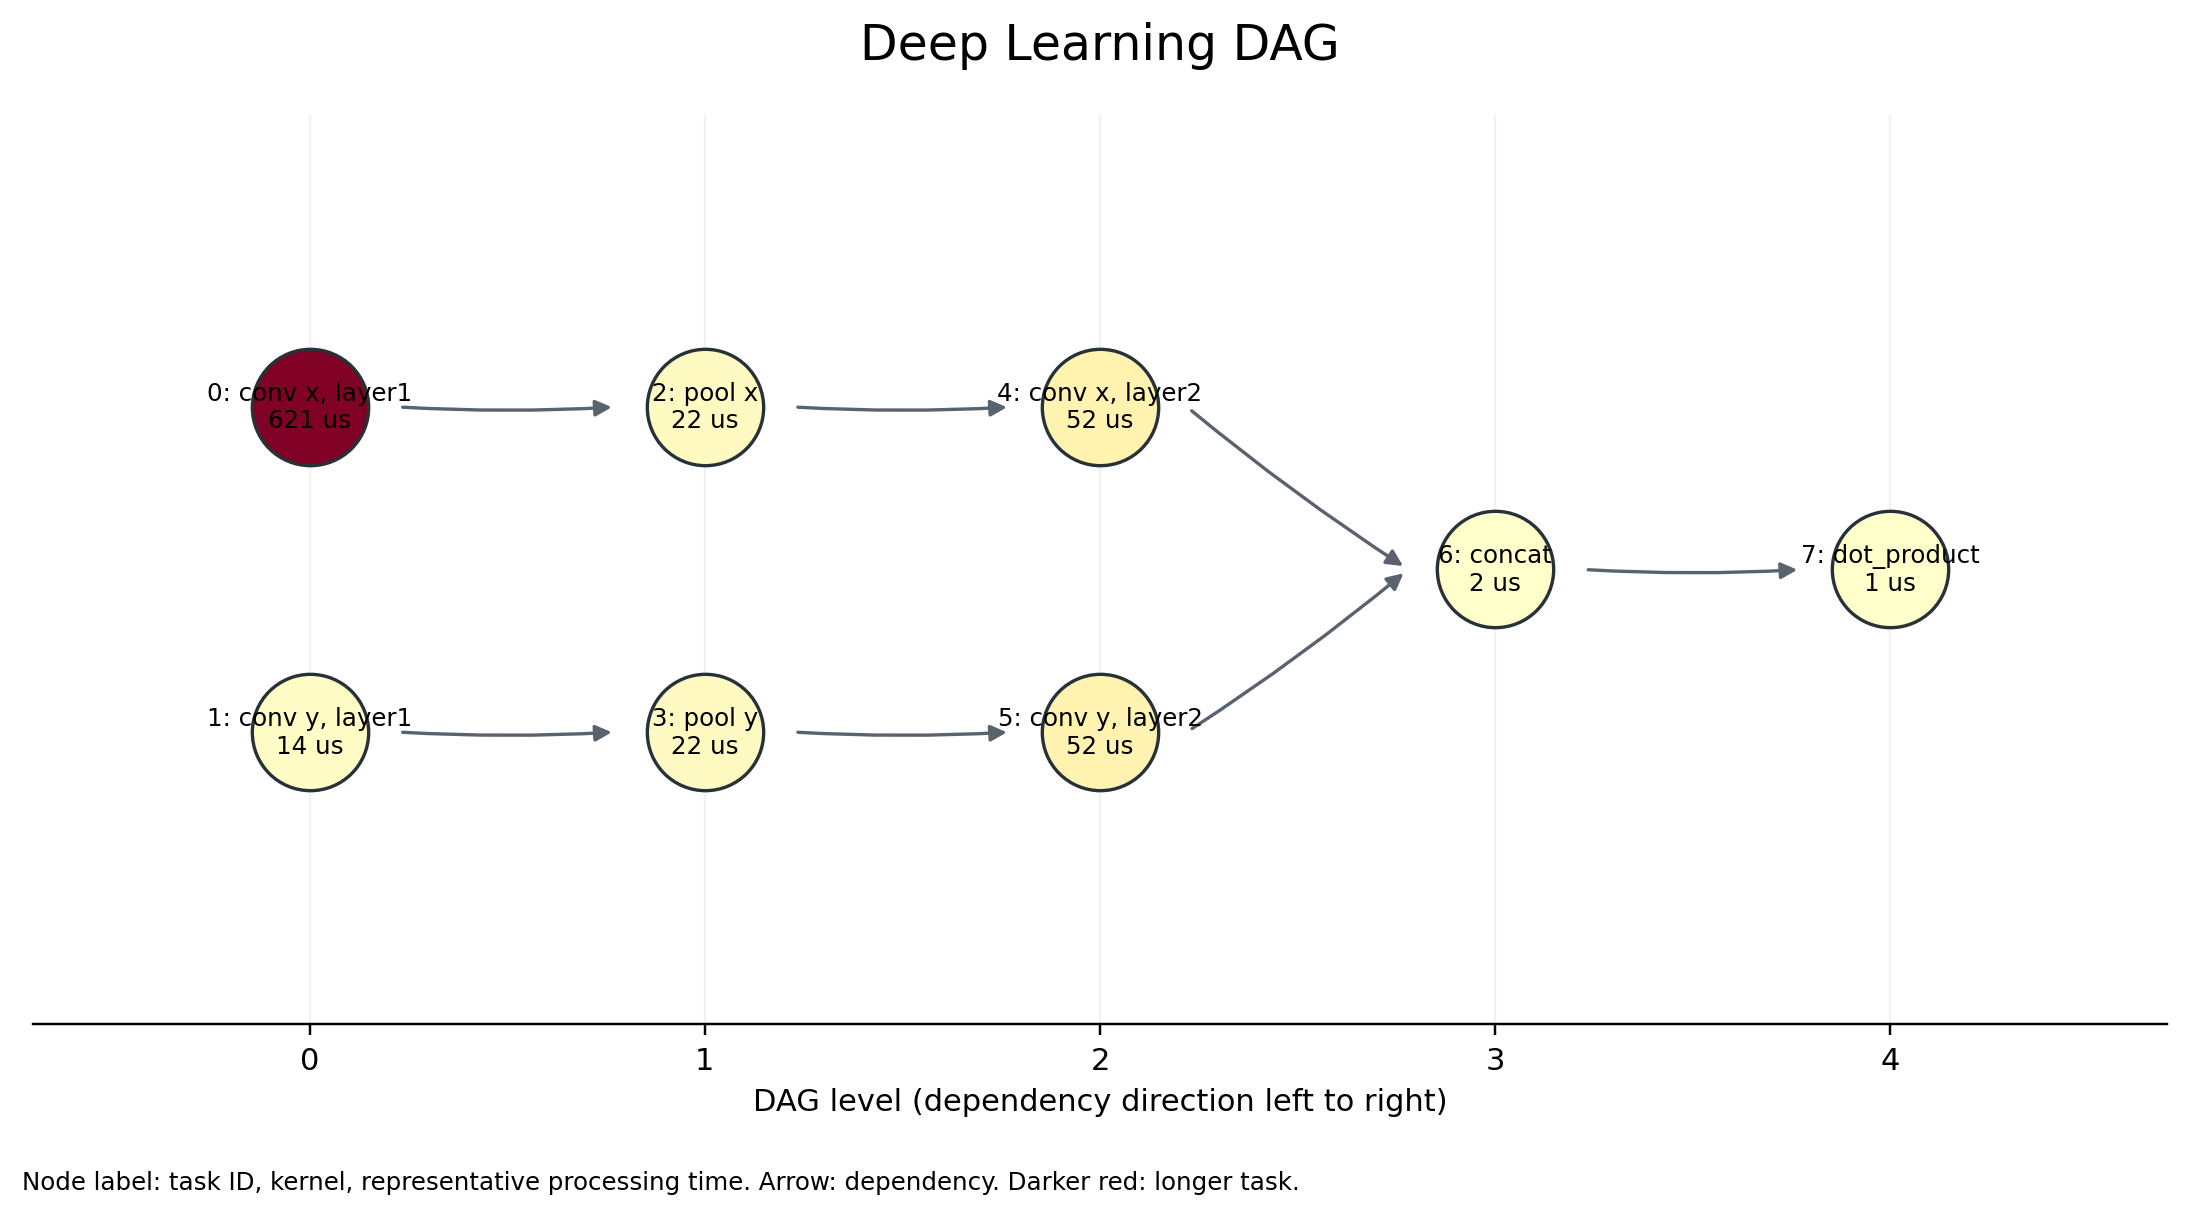
\includegraphics[width=\linewidth,height=0.43\textheight,keepaspectratio]{deep_learning_dag.png}
      \scriptsize
      \begin{tabular}{@{}lr@{}}
        根タスク数 / 最大幅 & 2 / 2 \\
        $W$ / $CP$ & 786 / 698 \\
        並列度上限 $W/CP$ & 1.13 \\
      \end{tabular}
      \par\smallskip
      \small 長い2分岐の遅い方を\code{concat}が待つ。
    \end{column}
  \end{columns}
\end{frame}

\begin{frame}{Stream数感度：多ければよいわけではない}
  \begin{columns}[T,onlytextwidth]
    \begin{column}{0.62\textwidth}
      \centering
      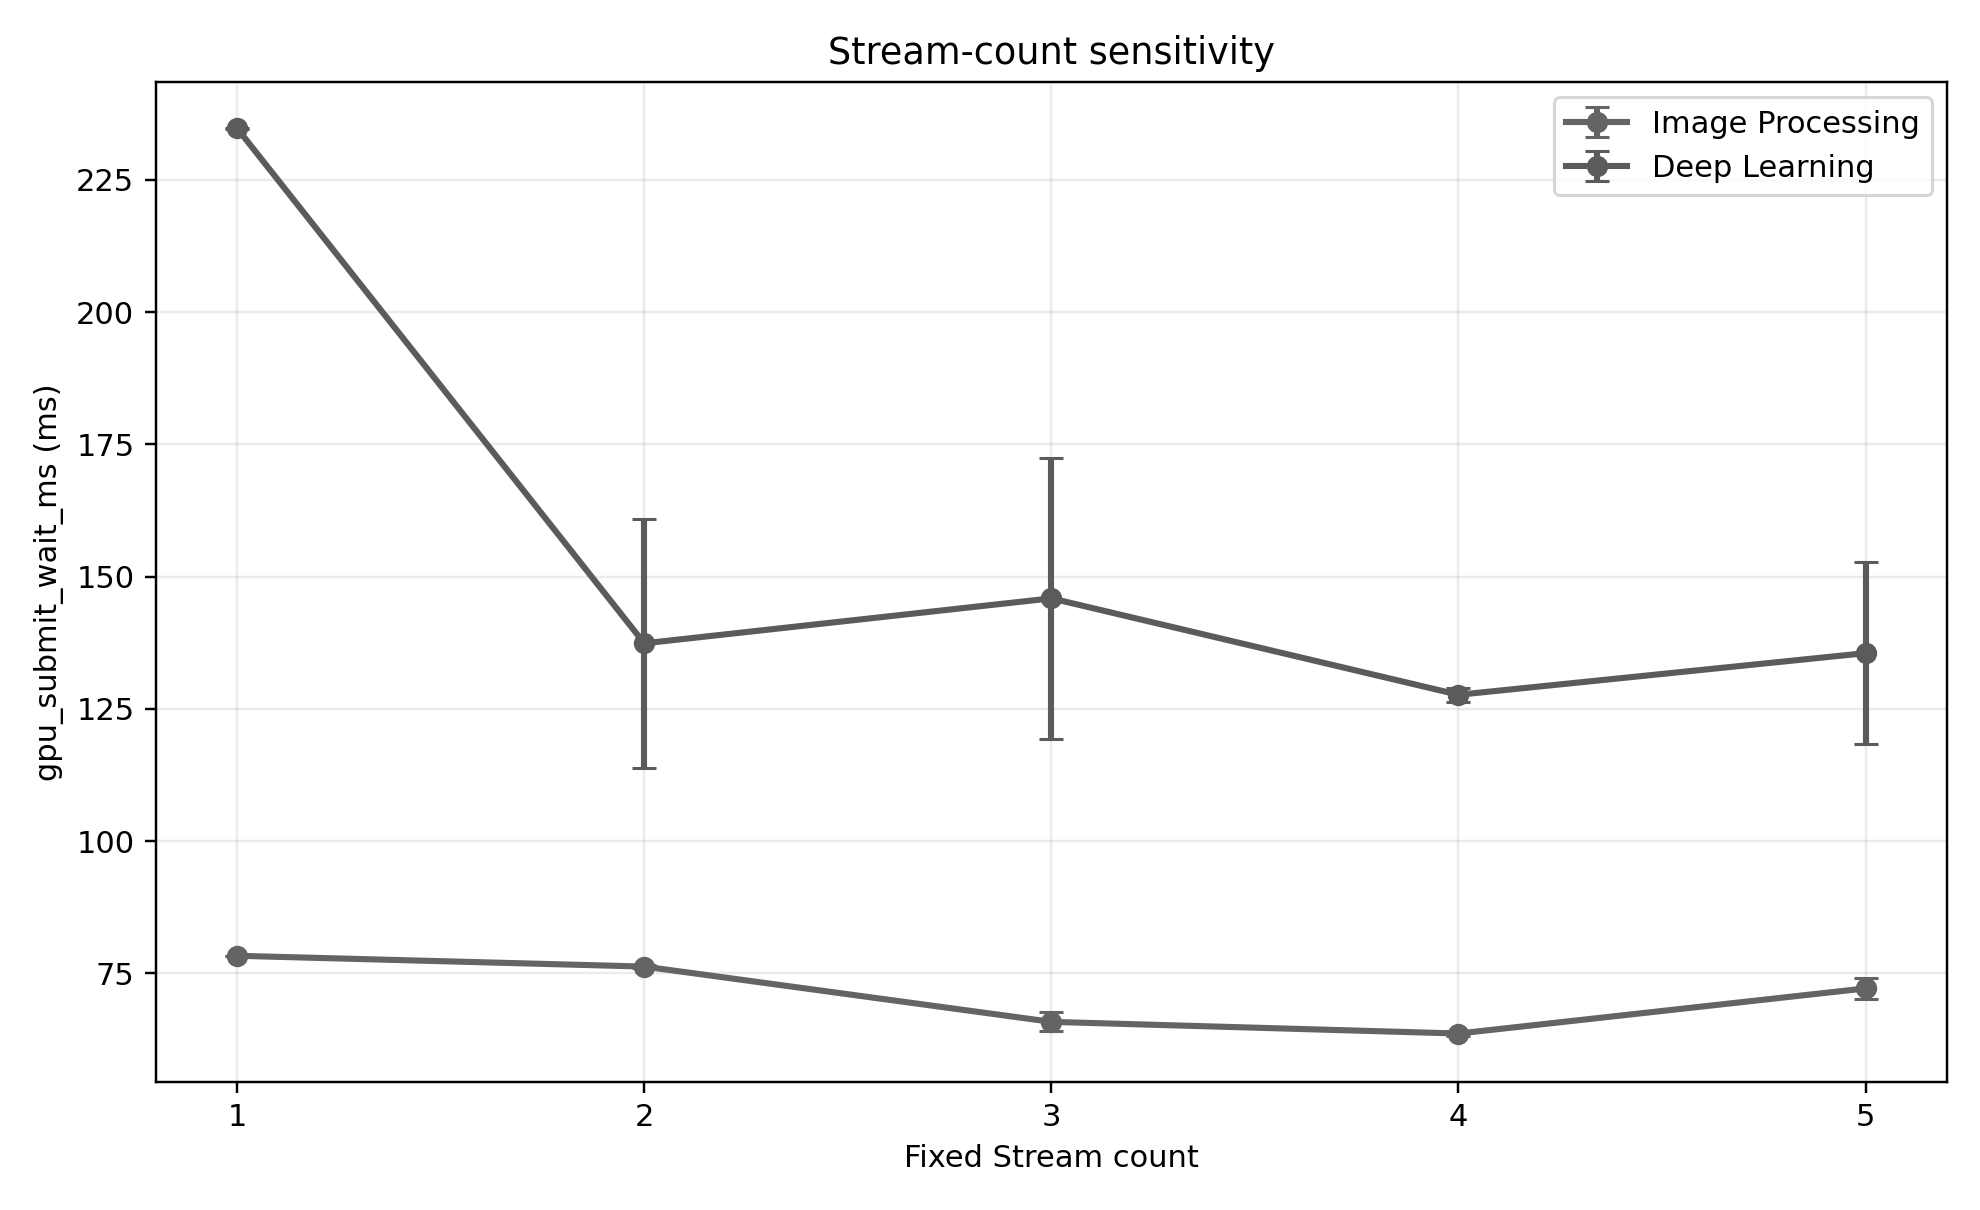
\includegraphics[width=\linewidth,height=0.66\textheight,keepaspectratio]{image_deep_stream_sensitivity.png}
    \end{column}
    \begin{column}{0.35\textwidth}
      \small
      \begin{block}{Image Processing}
        1 Stream: 78.23 ms\\
        \best{4 Streams: 63.45 ms}\\
        5 Streams: 71.97 ms
      \end{block}
      \begin{block}{Deep Learning}
        1 Stream: 234.64 ms\\
        \best{4 Streams: 127.52 ms}\\
        5 Streams: 135.39 ms
      \end{block}
      両者とも4 Streamが最短だが、提案方式全体が既存方式を上回るとは限らない。
    \end{column}
  \end{columns}
\end{frame}

\begin{frame}{厳密アブレーション：構成要素の寄与を分離}
  \begin{columns}[T,onlytextwidth]
    \begin{column}{0.62\textwidth}
      \centering
      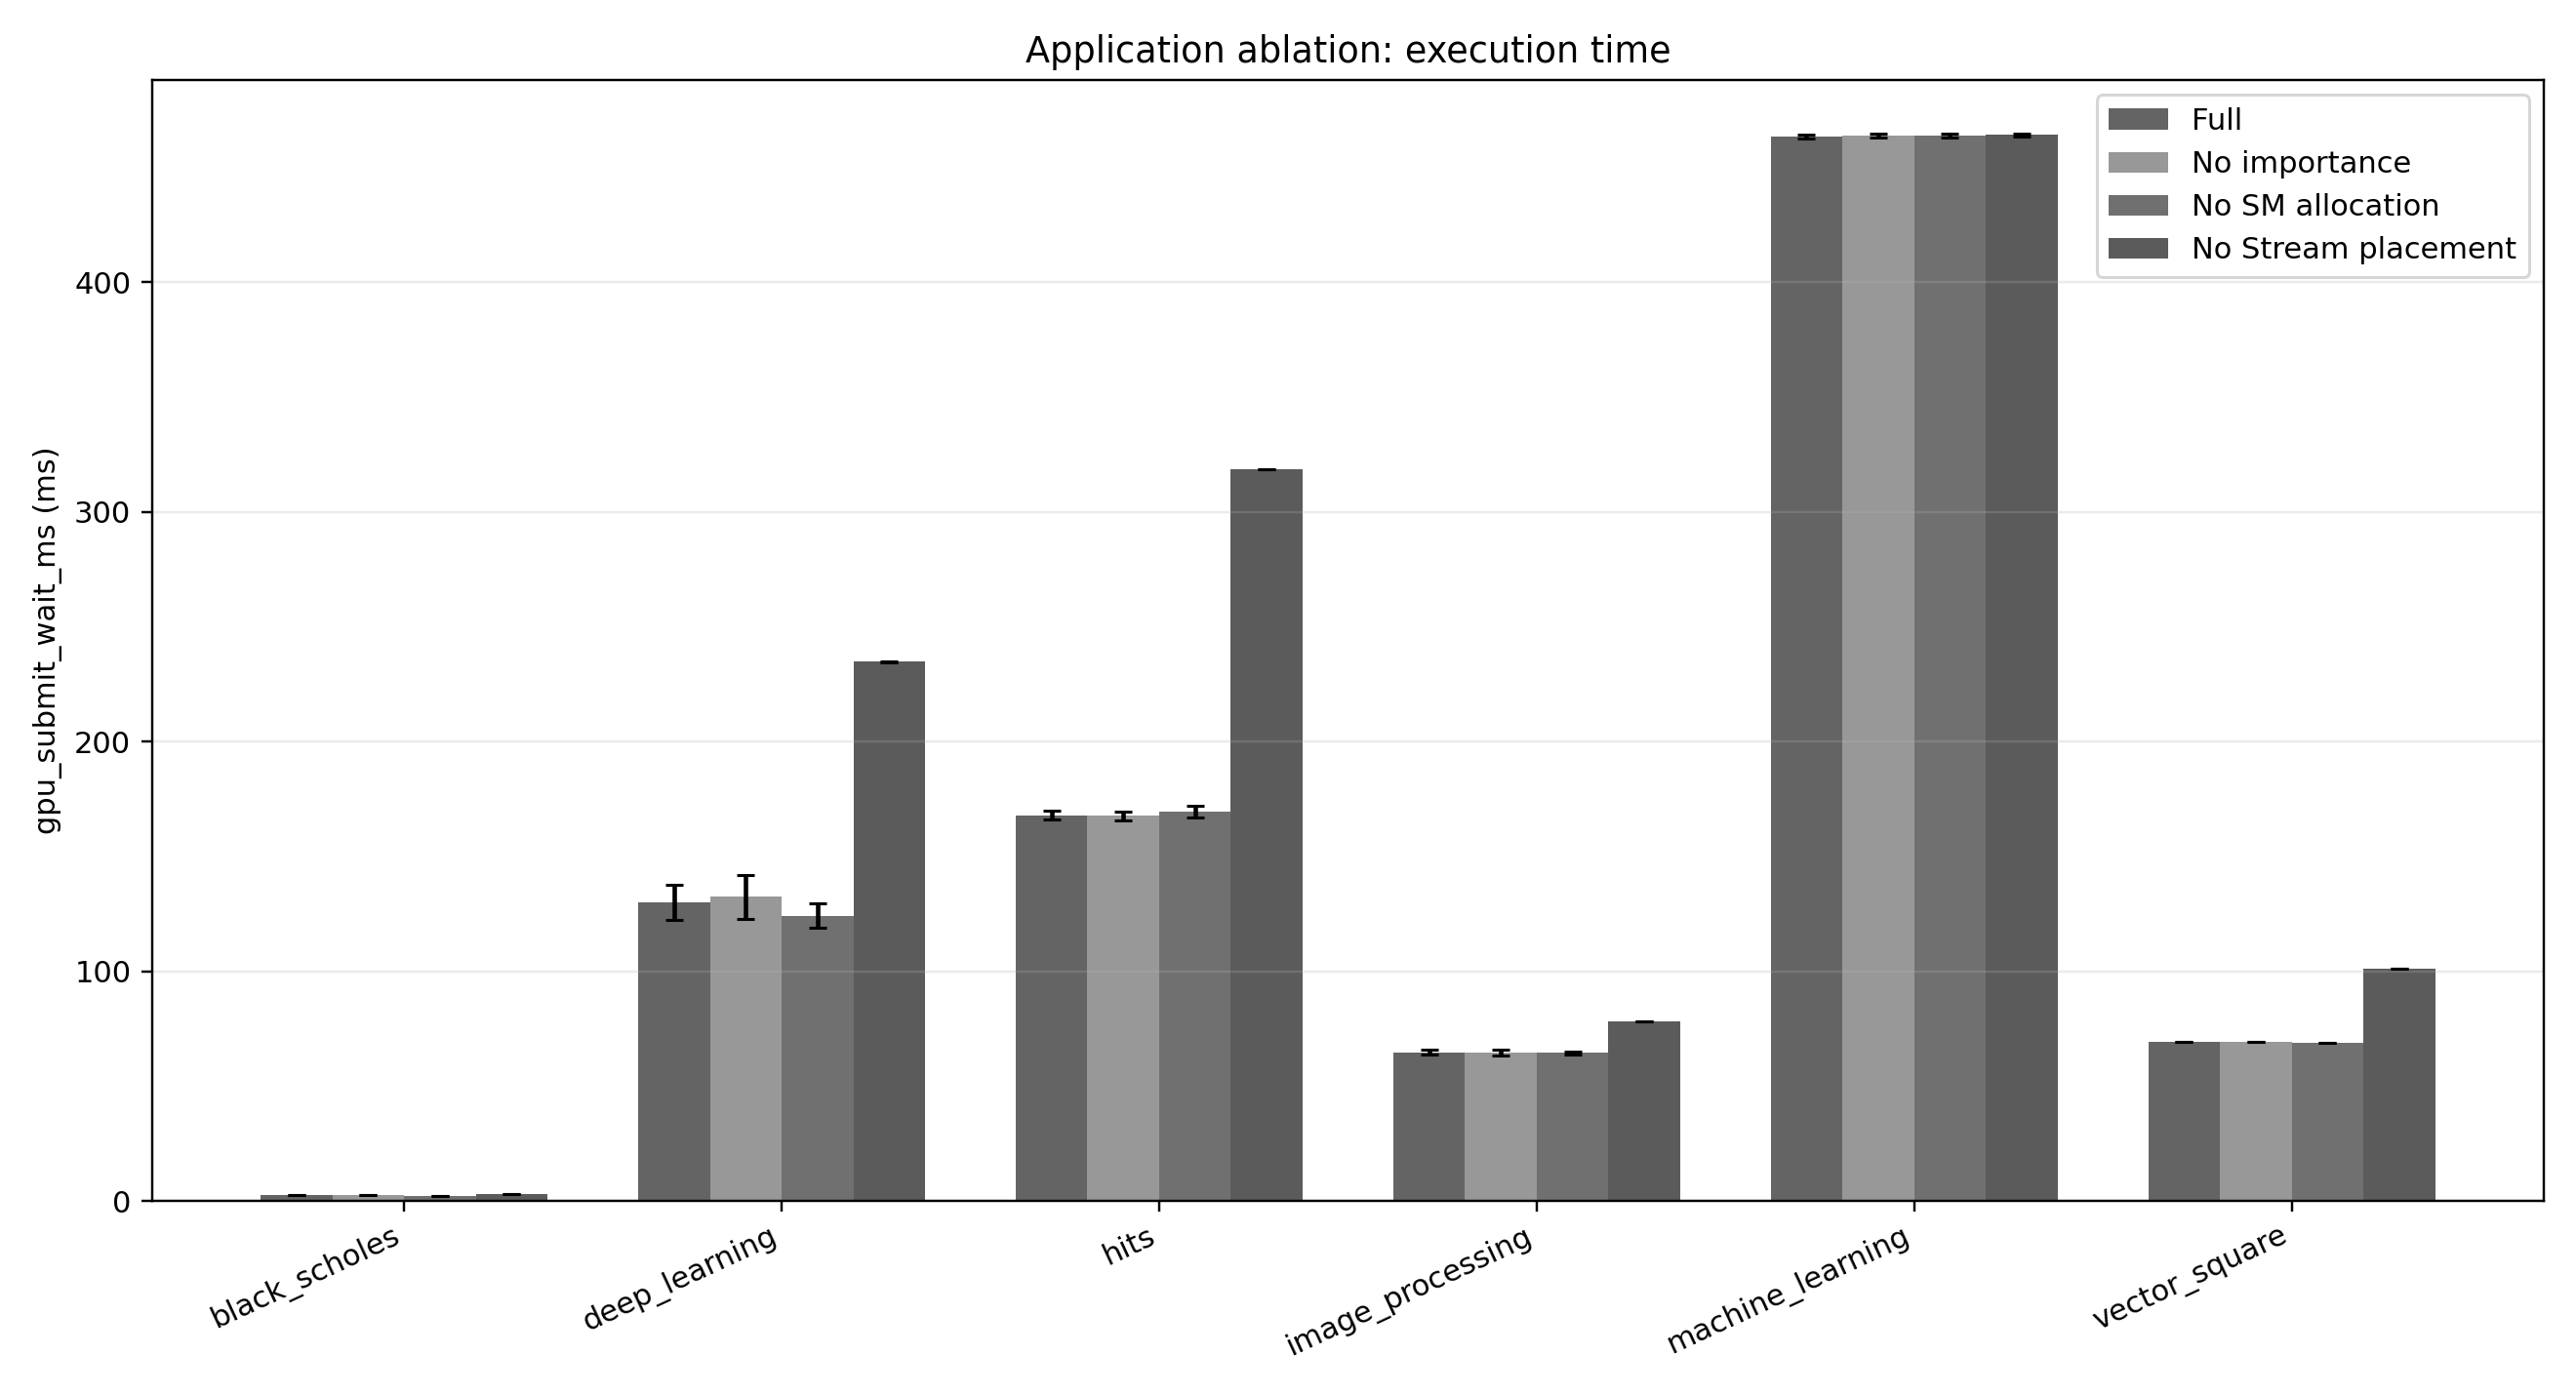
\includegraphics[width=\linewidth,height=0.68\textheight,keepaspectratio]{application_ablation_execution_time.png}
    \end{column}
    \begin{column}{0.35\textwidth}
      \small
      \begin{itemize}
        \item Full
        \item No importance
        \item No SM allocation
        \item No Stream placement
      \end{itemize}
      \begin{alertblock}{読み方}
        比較対象以外の入力・Stream数・測定方法を統一し、同じCUDA Event境界で比較する。
      \end{alertblock}
      Stream配置の効果は確認できる一方、重要度と非均等SM配分の追加効果は一様でない。
    \end{column}
  \end{columns}
\end{frame}

\begin{frame}{正確性と測定区間}
  \begin{columns}[T,onlytextwidth]
    \begin{column}{0.48\textwidth}
      \begin{block}{数値検証}
        \centering
        \Large \best{22 / 24 条件 PASS}
        \normalsize
        \par\medskip
        HITSのExisting・ProposedはFAIL。短い実行時間でも、結果が誤っていれば有効な性能値としない。
      \end{block}
      \begin{alertblock}{主指標}
        \code{gpu\_kernel\_ms}：最初のタスク開始から最後のタスク終了までのCUDA Event時間
      \end{alertblock}
    \end{column}
    \begin{column}{0.49\textwidth}
      \centering
      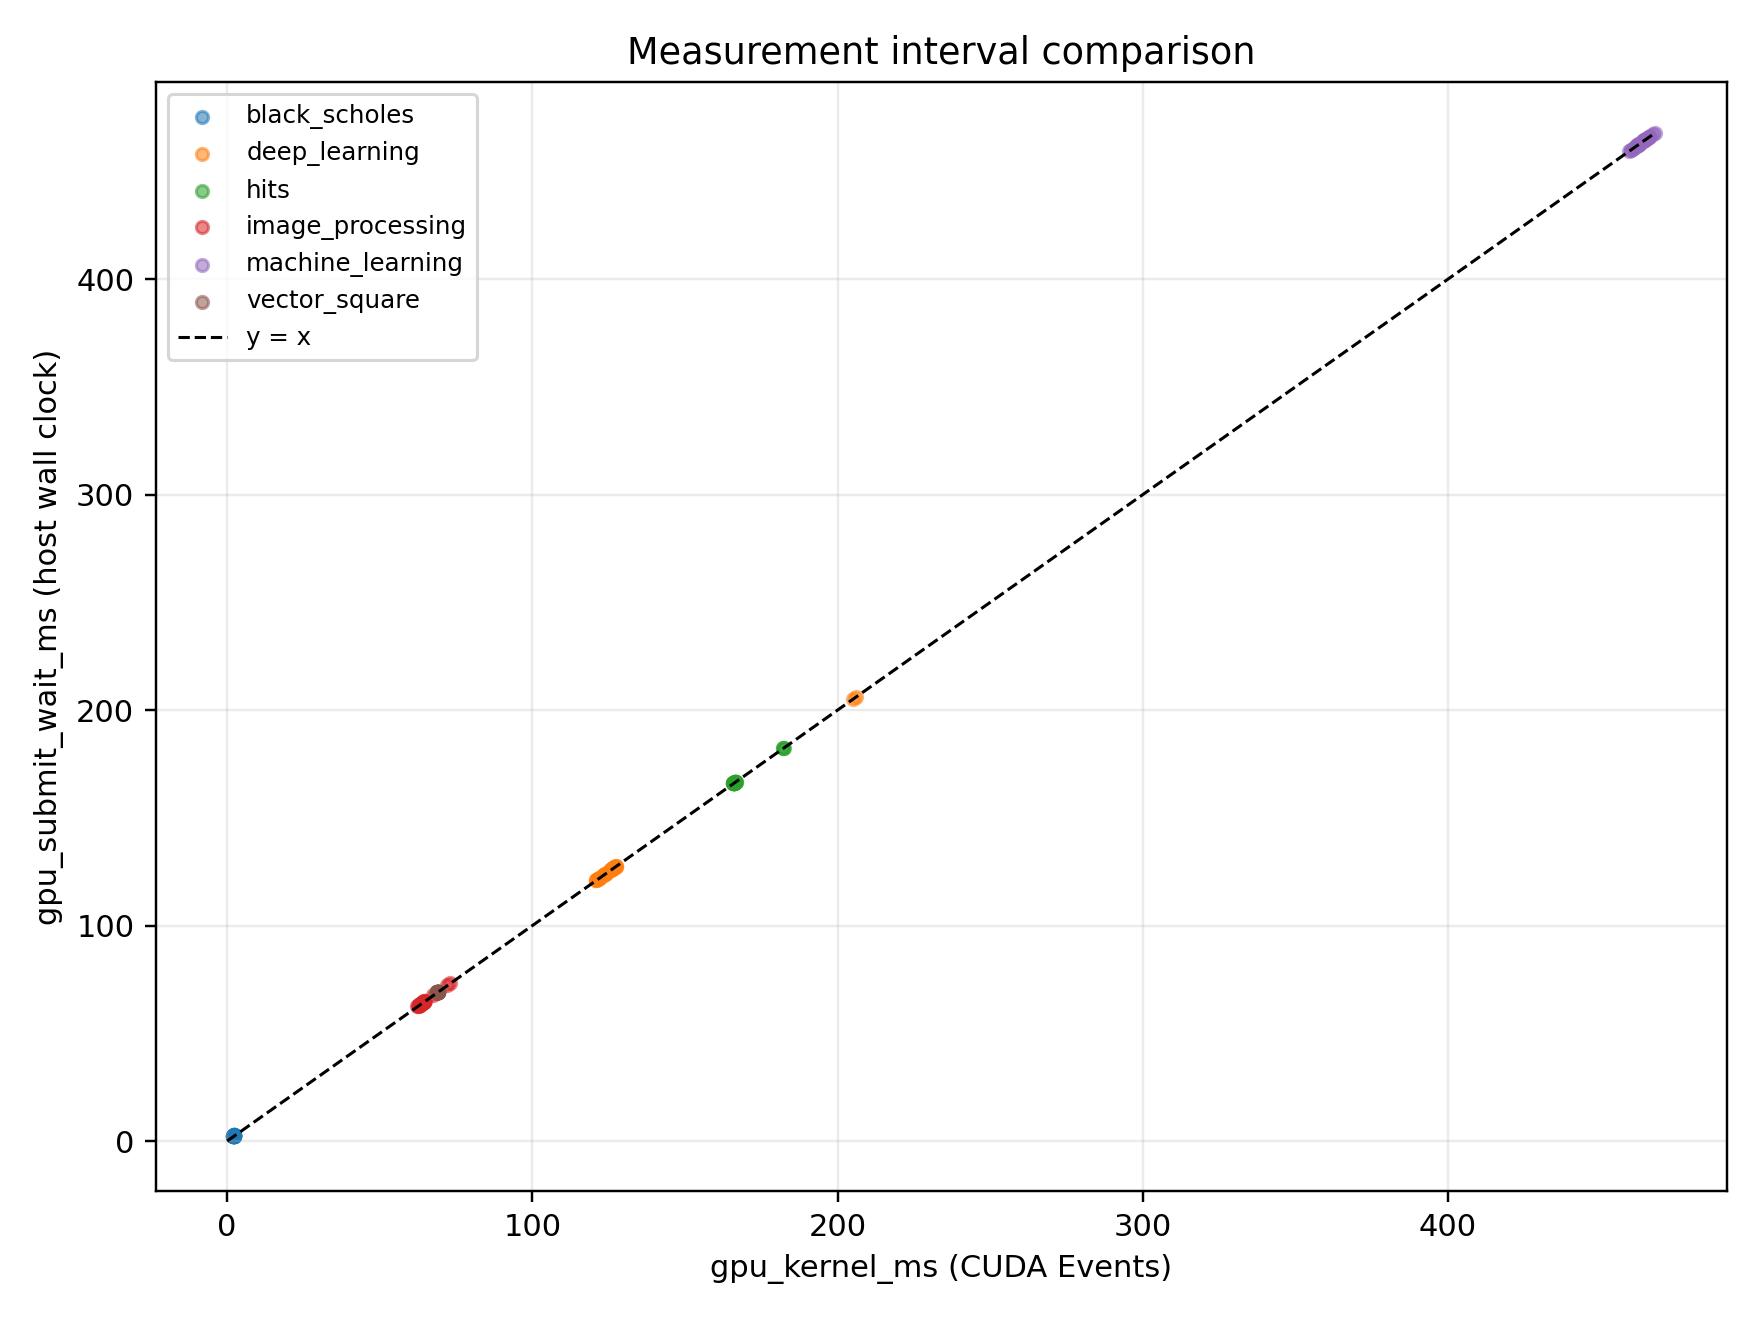
\includegraphics[width=\linewidth,height=0.65\textheight,keepaspectratio]{measurement_interval_comparison.png}
      \scriptsize
      \code{gpu\_submit\_wait\_ms}は投入・待機・資源解放・同期を含むホスト時間であり、主指標と分けて報告する。
    \end{column}
  \end{columns}
\end{frame}

\begin{frame}{スケジューリングオーバーヘッド}
  \centering
  \small
  \begin{tabular}{@{}lrrr@{}}
    \toprule
    ベンチマーク & Scheduling & GPU kernel & 比率 \\
    \midrule
    Black--Scholes   & 0.139 ms & 2.165 ms   & \caution{6.41\%} \\
    Deep Learning    & 0.129 ms & 129.900 ms & 0.10\% \\
    HITS             & 0.210 ms & 167.771 ms & 0.12\% \\
    Image Processing & 0.145 ms & 64.563 ms  & 0.22\% \\
    Machine Learning & 0.129 ms & 463.279 ms & 0.03\% \\
    Vector Square    & 0.120 ms & 68.920 ms  & 0.17\% \\
    \bottomrule
  \end{tabular}
  \vspace{5mm}
  \begin{itemize}
    \item 長時間実行ではGPU時間に対して0.03--0.22\%と小さい
    \item 短いBlack--Scholesでは6.41\%となり、無視できない
    \item 長時間または反復実行されるSTGで、結果を再利用する設計が適する
  \end{itemize}
\end{frame}

\begin{frame}{結論}
  \begin{block}{得られたこと}
    \begin{itemize}
      \item DAG重要度に基づくStream配置と、実測モデルによるSM配分を行う二段階ヒューリスティックを実装した
      \item 合成STGでは5種類すべてでProposedが最短だった
      \item 実アプリケーションではImage ProcessingのみProposedが最短で、最良方式は対象ごとに異なった
      \item 独立分岐が多いDAGではStream配置が効きやすく、長い分岐の合流では遅い分岐が支配的になる
    \end{itemize}
  \end{block}
  \begin{alertblock}{主張の範囲}
    提案方式は、DAG構造とカーネル特性に応じて配置・配分を構成的に決める方式であり、
    \caution{すべてのグラフで既存方式を上回る方式ではない}。
  \end{alertblock}
\end{frame}

\begin{frame}{限界と今後の課題}
  \begin{enumerate}
    \item グラフ規模評価を全サイズ・全seedで本計測する
    \item Random DAGを複数seedで集計し、平均と分散を報告する
    \item 複数GPU・異なる入力サイズでSM実測モデルを検証する
    \item 小規模グラフで全探索または整数計画法の最適解と比較する
    \item StreamごとのCUDA Event区間を測り、予測と実測の差を分析する
  \end{enumerate}
  \vspace{4mm}
  \begin{block}{主張しないこと}
    「どのグラフでも最速」「SM使用率最大ならmakespan最小」
    「GPUや入力に依存せず有効」「厳密最適解を求める」
  \end{block}
\end{frame}

\begin{frame}[plain]
  \centering
  \vfill
  {\LARGE まとめ}\par\medskip
  {\large 性能を決めるのはStream数だけではない。}\par\medskip
  {\large \textbf{DAG構造、クリティカルパス、実カーネルのSM特性}を\\
  一体として扱う必要がある。}
  \vfill
\end{frame}

% 付録：分野横断の関連手法。直接比較候補と設計原理だけが類似する
% 方式を混同しないため、比較単位と相違点を明記する。
\appendix
\section{付録：分野横断の関連手法}

\begin{frame}{付録の比較基準：提案手法 $P$}
  \small
  \begin{block}{問題設定}
    静的DAG上の非プリエンプティブCUDAカーネルを単一GPUで実行し、
    実測または合成のSM--時間モデルを用いてmakespanを短縮する。
  \end{block}
  \begin{enumerate}
    \item $BL(i)=p_i+\max_{j\in succ(i)}BL(j)$ によりreadyタスクを順位付け
    \item 既配置区間への挿入を含むEFT最小のStreamへ配置
    \item 1--5 Streamについて配置を生成
    \item 配置を固定し、合計114 SMを原則8 SM単位で配分探索
    \item SM依存実行時間でDAGとStream直列化を再評価し、予測makespan最小を選択
  \end{enumerate}
  \begin{alertblock}{比較で必ず区別する点}
    DAGの有無、静的/動的、プリエンプション、目的関数、実行先選択、
    資源量による処理時間変化、配置後の資源再配分、通信コストの有無。
  \end{alertblock}
\end{frame}

\begin{frame}{CPU・プロセス：HLFET、ETF、MCP}
  \scriptsize
  \begin{block}{HLFET（直接類似：高）}
    \textbf{概要：}DAGの後続経路長に基づく静的レベルが高いタスクからプロセッサへ配置する。\par
    \textbf{$P$との差：}プロセッサ内部の計算資源量を配置後に変更しない。$P$はStream配置後に
    SM数を探索し、SM数による処理時間変化も再評価する。
  \end{block}
  \begin{block}{ETF（直接類似：高）}
    \textbf{概要：}readyなタスク--プロセッサ対の開始・完了時刻を比較し、最早の組を選ぶ。\par
    \textbf{$P$との差：}ETFは対を一体として選ぶのに対し、$P$は先にbottom level最大のタスクを
    固定し、そのタスクについて挿入型EFT最小のStreamを選ぶ。
  \end{block}
  \begin{block}{MCP（直接類似：中--高）}
    \textbf{概要：}ALAP時刻等からクリティカルなタスク順を構成し、依存経路を重視して割り当てる。\par
    \textbf{$P$との差：}優先度定義がbottom levelと同一ではなく、固定能力のプロセッサを前提とする。
    $P$は明示的なクリティカルパス固定ではなく、全readyタスクをBLで順位付けする。
  \end{block}
\end{frame}

\begin{frame}{リアルタイム：EDF、LLF、DAG-EDF}
  \scriptsize
  \begin{block}{EDF（類推：低）}
    \textbf{概要：}絶対締切が最も早いreadyジョブを優先する。\par
    \textbf{$P$との差：}優先度はdeadlineでありDAGの後続経路長ではない。目的はdeadline miss回避で、
    $P$の単一DAG makespan最小化とは異なる。動的・プリエンプティブにも使われる。
  \end{block}
  \begin{block}{LLF（類推：低--中）}
    \textbf{概要：}締切までの余裕から残り処理時間を引いたlaxity最小のジョブを優先する。\par
    \textbf{$P$との差：}LLF優先度は時刻とともに変化するが、$P$のBLは実行前に固定される。
    LLFはdeadlineを扱い、Stream選択・SM配分を含まない。
  \end{block}
  \begin{block}{DAG-EDF（構造類似：中）}
    \textbf{概要：}先行制約を満たしたDAGノードをEDF規則で複数プロセッサへ投入する方式群。\par
    \textbf{$P$との差：}DAG-EDFはDAGジョブのdeadline保証が中心で、オンライン判断を含み得る。
    $P$は個別deadlineを持たず、静的配置とSM構成をmakespanで選ぶ。
  \end{block}
\end{frame}

\begin{frame}{並列・分散計算：HEFT、CPOP、PEFT}
  \scriptsize
  \begin{block}{HEFT（最重要の直接類似）}
    \textbf{概要：}平均計算・通信コストによるupward rank順に、挿入型EFT最小の異種プロセッサへ配置する。\par
    \textbf{$P$との差：}HEFTは配置時から実行先別時間と通信費を用いる。$P$のStage 3は共通$p_i$でStreamを選び、
    配置後にSM依存時間でStream数・SM数を探索する。$P$は通信コストを明示的に持たない。
  \end{block}
  \begin{block}{CPOP（直接類似：高）}
    \textbf{概要：}upward/downward rankからクリティカルパスを特定し、パスタスクを選択プロセッサへ集約する。\par
    \textbf{$P$との差：}$P$はクリティカルパスを抽出・同一Streamへ固定せず、重要タスクもEFTにより分散し得る。
    CPOPには配置後のSM分割探索がない。
  \end{block}
  \begin{block}{PEFT（直接類似：非常に高）}
    \textbf{概要：}Optimistic Cost Tableでタスク--プロセッサ別の将来コストを計算し、順位と配置に用いる。\par
    \textbf{$P$との差：}PEFTは配置時に実行先別の後続コストを先読みするが、$P$のBLはStream非依存である。
    一方$P$は配置後に離散SM配分を全探索する。
  \end{block}
\end{frame}

\begin{frame}{クラウド・コンテナ：Kubernetes、Firmament、DRF}
  \scriptsize
  \begin{block}{Kubernetes Filter--Score（構造類似：低--中）}
    \textbf{概要：}資源・制約を満たさないNodeを除外し、残るNodeを複数規則で採点してPodを配置する。\par
    \textbf{$P$との差：}標準方式はPod間DAGやクリティカルパスを直接扱わず、オンラインで1 Podずつ配置する。
    目的も必ずしもmakespanではなく、配置後の全体SM再配分は行わない。
  \end{block}
  \begin{block}{Firmament（構造類似：中以下）}
    \textbf{概要：}クラスタ配置をmin-cost max-flowとして表し、監視イベントに応じて全タスクを継続的に再最適化する。\par
    \textbf{$P$との差：}大規模クラスタの大域的・動的配置であり、BL順の貪欲構築ではない。
    目的はポリシー依存の配置コストで、単一DAG makespanに限定されない。
  \end{block}
  \begin{block}{DRF（類推：低）}
    \textbf{概要：}CPU・メモリ等についてユーザーのdominant shareを均等化する多資源公平配分。\par
    \textbf{$P$との差：}目的は公平性でDAGを扱わない。$P$は主に単一資源SMを不均等配分してmakespanを下げるため、
    ユーザー間公平性は目的としない。
  \end{block}
\end{frame}

\begin{frame}{ジョブ・ワークフロー：DLS、Min--Min、方式群}
  \scriptsize
  \begin{block}{DLS（直接類似：高）}
    \textbf{概要：}後続経路由来の静的重要度と、実行先別の早期開始効果をdynamic levelへ統合し、
    タスク--プロセッサ対を選ぶ。\par
    \textbf{$P$との差：}DLSは対を同時に選び、異種性能・通信費を配置時に扱う。$P$はBLでタスクを先に選び、
    EFTでStreamを決めた後、SM量を別段階で探索する。
  \end{block}
  \begin{block}{Min--Min（構造類似：中）}
    \textbf{概要：}未割当てタスクごとの最小完了時刻を求め、その値が最小のタスクを先に配置する。\par
    \textbf{$P$との差：}通常は独立タスクを対象とし短いタスクを優先しやすい。$P$はDAGの後続を含むBLが大きい
    タスクを優先し、配置後に資源能力も変える。
  \end{block}
  \begin{block}{Heterogeneous Critical Path Scheduling（名称上の注意）}
    \textbf{概要：}異種環境でクリティカルパスを利用する方式の総称で、単一の標準アルゴリズムではない。\par
    \textbf{$P$との差：}数式レベルの比較対象を一意に定められない。論文ではこの総称をベースライン名にせず、
    HEFT、CPOP、PEFT等の具体的方式へ置換する。
  \end{block}
\end{frame}

\begin{frame}{ネットワーク：Packet EDF、WFQ、DRR}
  \scriptsize
  \begin{block}{Packet EDF（類推：低）}
    \textbf{概要：}deadlineが最も近いパケットを先に送信するオンラインキュー制御。\par
    \textbf{$P$との差：}通常はパケット間DAGを持たず、目的は期限遵守である。$P$は非プリエンプティブな
    カーネルDAG全体のmakespanと実行構成を実行前に決める。
  \end{block}
  \begin{block}{WFQ（類推：低）}
    \textbf{概要：}フローの重みに比例してリンク帯域を公平に共有する。\par
    \textbf{$P$との差：}公平性・遅延保証が中心で、BLやEFTを用いない。$P$は重要Streamへ多くのSMを与え得る
    離散的静的配分であり、公平性を要求しない。
  \end{block}
  \begin{block}{DRR（類推：低）}
    \textbf{概要：}各キューへquantumを与え、不足分を次巡へ繰り越す低計算量の公平キューイング。\par
    \textbf{$P$との差：}巡回型オンライン方式であり、依存グラフや全体makespanを扱わない。
    $P$のSM配分は一度決める固定構成で、実行中に量子を繰り越さない。
  \end{block}
\end{frame}

\begin{frame}{データベース：クリティカル経路、SRPT、Eddy}
  \scriptsize
  \begin{block}{Critical-path Query Scheduling（方式群）}
    \textbf{概要：}クエリDAG中のクリティカル演算子やパイプラインを優先する考え方の総称。\par
    \textbf{$P$との差：}クエリではデータ量変化、I/O、パイプライン処理が支配的で、固定$p_i$の非プリエンプティブ
    カーネルとは異なる。特定論文・方式を指定しない限り正式ベースラインにはできない。
  \end{block}
  \begin{block}{SRPT（類推：低）}
    \textbf{概要：}残り処理時間が最小のジョブを優先し、平均応答時間を短縮する。\par
    \textbf{$P$との差：}短いジョブを優先するため、長い後続経路を持つタスクを優先する$P$と逆の選択になり得る。
    通常はDAG・実行先選択・SM配分を扱わず、プリエンプティブである。
  \end{block}
  \begin{block}{Eddy（構造類似：低--中）}
    \textbf{概要：}実行時の選択度やキュー状態により、タプルを次の演算子へ動的ルーティングする。\par
    \textbf{$P$との差：}Eddyはタプル単位の適応的実行で、$P$はカーネル単位の静的配置である。
    $P$は事前測定モデルを使い、実行中の観測による再ルーティングをしない。
  \end{block}
\end{frame}

\begin{frame}{製造・生産：Shifting Bottleneck、CR、LPT}
  \scriptsize
  \begin{block}{Shifting Bottleneck Procedure（構造類似：中--高）}
    \textbf{概要：}最も重大なボトルネック機械を選び、その機械上の順序を固定し、既決定部分も再最適化する。\par
    \textbf{$P$との差：}独立機械のdisjunctive graphを反復改善する方式である。$P$は既定DAG上で配置を一度構築し、
    同一GPUを分割したStreamのSM量だけを配置後に探索する。
  \end{block}
  \begin{block}{Critical Ratio（類推：低）}
    \textbf{概要：}納期までの残時間を残り処理時間で割った比により、余裕の小さいジョブを優先する。\par
    \textbf{$P$との差：}時刻・納期依存の優先度でDAG後続長を使わず、実行先・資源量も選ばない。
    $P$はdeadlineを入力に持たない。
  \end{block}
  \begin{block}{LPT（構造類似：中）}
    \textbf{概要：}長い独立ジョブから負荷の小さい固定能力機械へ配置し、makespanを抑える。\par
    \textbf{$P$との差：}$P$は自身の長さではなく後続経路を含むBLを使う。さらにDAG先行制約があり、
    Stream能力もSM配分で変化する。
  \end{block}
\end{frame}

\begin{frame}{人員・勤務表：優先規則、CP、GA}
  \scriptsize
  \begin{block}{Priority-rule Scheduling（方式群、構造類似：中）}
    \textbf{概要：}資格、重要度、希望、締切等から作業を順位付けし、順次人員へ割り当てる。\par
    \textbf{$P$との差：}一意のアルゴリズムではなく、公平性・労働時間・資格等の多制約が中心である。
    $P$はBLという固定規則、先行制約、SM総量、makespanを中心とする。
  \end{block}
  \begin{block}{Constraint Programming（探索枠組み、類似：低）}
    \textbf{概要：}hard/soft制約を宣言し、制約伝播と分枝探索で勤務表を求める。\par
    \textbf{$P$との差：}CPは汎用探索で最適性を証明できる場合がある。$P$の配置は専用の貪欲法であり、
    SM配分だけを限定候補内で全探索するため、全体最適性を保証しない。
  \end{block}
  \begin{block}{Genetic Algorithm（探索枠組み、類似：低）}
    \textbf{概要：}勤務表を個体とし、交叉・突然変異・選択で多目的評価を反復改善する。\par
    \textbf{$P$との差：}GAは確率的で配置自体を繰り返し変更する。$P$は決定的な一方向配置で、
    固定配置に対する離散SM配分のみ網羅する。
  \end{block}
\end{frame}

\begin{frame}{交通・物流：VRPTW挿入、ALNS、CR dispatching}
  \scriptsize
  \begin{block}{VRPTW Insertion Heuristic（構造類似：中）}
    \textbf{概要：}時間窓・容量を満たしながら、追加距離または終了時刻増分が小さい車両・位置へ配送を挿入する。\par
    \textbf{$P$との差：}移動距離、時間窓、車両容量を扱い、DAG先行制約やSM数は扱わない。
    共通するのは既存区間の可行な空き位置へ貪欲挿入する部分である。
  \end{block}
  \begin{block}{ALNS（改善候補、直接類似：低）}
    \textbf{概要：}解の一部を破壊・再構築し、複数の近傍操作を適応的に選択する。\par
    \textbf{$P$との差：}ALNSは配置自体を反復改善し局所最適から脱出するが、$P$はStage 3配置を固定したまま
    Stage 4へ進む。将来の配置改善法としては利用可能である。
  \end{block}
  \begin{block}{Critical-ratio Dispatching（方式群、類似：低）}
    \textbf{概要：}納期余裕と残り作業量から遅延危険の高い配送・車両を優先する。\par
    \textbf{$P$との差：}DAGの後続経路や実行先能力の探索を含まない。固有の単一物流方式ではないため、
    正式比較には具体的な問題設定と文献の指定が必要である。
  \end{block}
\end{frame}

\begin{frame}{教育・施設予約：DSATUR、LDF、Tabu Search}
  \scriptsize
  \begin{block}{DSATUR（構造類似：低--中）}
    \textbf{概要：}隣接頂点で既使用の色数が最大の頂点を優先するグラフ彩色ヒューリスティック。\par
    \textbf{$P$との差：}無向競合グラフ上の色数・競合最小化で、処理時間や有向依存を持たない。
    共通するのは制約が厳しい対象を優先する決定的貪欲構築のみである。
  \end{block}
  \begin{block}{Largest-Degree-First（類似：低）}
    \textbf{概要：}競合辺が多い授業から時間枠へ割り当てる。\par
    \textbf{$P$との差：}優先度は無向グラフ次数で、$P$の重み付き有向後続最長路とは異なる。
    資源能力や処理時間を配置後に変更しない。
  \end{block}
  \begin{block}{Tabu Search Timetabling（類似：低）}
    \textbf{概要：}授業の移動・交換を行い、Tabuリストで循環を避けつつ制約違反を反復削減する。\par
    \textbf{$P$との差：}soft constraintを含む局所探索で、構築後も配置を変更する。
    $P$は単一主要目的の決定的構築で、配置の近傍探索を行わない。
  \end{block}
\end{frame}

\begin{frame}{プロジェクト管理：CPM、SSGS、PSGS}
  \scriptsize
  \begin{block}{CPM（分析上の類似：高）}
    \textbf{概要：}DAGの最早・最遅時刻を計算し、余裕ゼロのクリティカルパスを特定する。\par
    \textbf{$P$との差：}標準CPMは資源競合を無視する分析法で、実行先配置を生成しない。
    $P$は同種の後向き長さを優先度に使い、Stream競合とSM容量を含む実行構成を生成する。
  \end{block}
  \begin{block}{SSGS（構造類似：非常に高）}
    \textbf{概要：}eligible作業から優先規則で1件を選び、先行・資源制約を満たす最早位置へ配置する。\par
    \textbf{$P$との差：}SSGSは生成方式であり優先規則は外部指定、通常は作業の資源要求が固定である。
    $P$はBLを規則として固定し、Stream順序資源に加えてSM量で処理時間も変える。
  \end{block}
  \begin{block}{PSGS（構造類似：高）}
    \textbf{概要：}時間を進め、その時点でreadyかつ資源可行な複数作業を並列開始する。\par
    \textbf{$P$との差：}PSGSは時間軸を進めるイベント型だが、$P$は1タスクずつ将来区間へ挿入する。
    $P$のStage 3はPSGSよりSSGSに近く、その後にSM配分段階を持つ。
  \end{block}
\end{frame}

\begin{frame}{関連手法から導く本研究の厳密な位置付け}
  \small
  \begin{block}{位置付け}
    本手法は、\textbf{HEFT型のDAGリストスケジューリング}を単一GPU内のCUDA Stream配置へ適用し、
    その配置を固定した後に、\textbf{カーネル別SMスケーリングモデル}を用いて
    Stream数とStream別SM数を探索する二段階静的ヒューリスティックである。
  \end{block}
  \begin{alertblock}{独自性を主張するために残る検証}
    \begin{enumerate}
      \item 同一GPU・同一時間モデルで実装したHEFT/PEFTとの比較
      \item 配置とSM配分を同時探索する最適解または下界との比較
      \item 通信費なし・同種Streamという条件で、BL+EFT自体の新規性とSM探索の寄与を分離
      \item 配置固定が最終SM配分に対して不利になる反例と性能差の測定
    \end{enumerate}
  \end{alertblock}
  \begin{exampleblock}{直接ベースラインとして推奨}
    HEFT、PEFT、CPOP、DLS、均等SM、SM配分なし、importanceなし、配置なし。
  \end{exampleblock}
\end{frame}

\begin{frame}{関連研究の主要文献}
  \tiny
  \begin{thebibliography}{9}
    \bibitem{heft} H.~Topcuoglu, S.~Hariri, and M.-Y.~Wu,
      ``Performance-Effective and Low-Complexity Task Scheduling for Heterogeneous Computing,''
      \emph{IEEE TPDS}, 13(3), 2002. DOI: 10.1109/71.993206.
    \bibitem{peft} H.~Arabnejad and J.~G.~Barbosa,
      ``List Scheduling Algorithm for Heterogeneous Systems by an Optimistic Cost Table,''
      \emph{IEEE TPDS}, 25(3), 2014. DOI: 10.1109/TPDS.2013.57.
    \bibitem{dls} G.~C.~Sih and E.~A.~Lee,
      ``A Compile-Time Scheduling Heuristic for Interconnection-Constrained Heterogeneous Processor Architectures,''
      \emph{IEEE TPDS}, 4(2), 1993.
    \bibitem{drf} A.~Ghodsi et al., ``Dominant Resource Fairness: Fair Allocation of Multiple Resource Types,''
      \emph{NSDI}, 2011.
    \bibitem{firmament} I.~Gog et al., ``Firmament: Fast, Centralized Cluster Scheduling at Scale,''
      \emph{OSDI}, 2016.
    \bibitem{sbp} J.~Adams, E.~Balas, and D.~Zawack,
      ``The Shifting Bottleneck Procedure for Job Shop Scheduling,'' \emph{Management Science}, 34(3), 1988.
    \bibitem{sgs} R.~Kolisch,
      ``Serial and Parallel Resource-Constrained Project Scheduling Methods Revisited,''
      \emph{European Journal of Operational Research}, 90(2), 1996.
  \end{thebibliography}
  \vspace{-2mm}
  \begin{alertblock}{注記}
    ``Heterogeneous Critical Path Scheduling''、``Critical-path Query Scheduling''、
    ``Priority-rule Scheduling''等は単一方式名ではないため、本文で用いる場合は具体的論文へ置き換える。
  \end{alertblock}
\end{frame}

\end{document}
